% Options for packages loaded elsewhere
\PassOptionsToPackage{unicode}{hyperref}
\PassOptionsToPackage{hyphens}{url}
%
\documentclass[
]{article}
\usepackage{amsmath,amssymb}
\usepackage{iftex}
\ifPDFTeX
  \usepackage[T1]{fontenc}
  \usepackage[utf8]{inputenc}
  \usepackage{textcomp} % provide euro and other symbols
\else % if luatex or xetex
  \usepackage{unicode-math} % this also loads fontspec
  \defaultfontfeatures{Scale=MatchLowercase}
  \defaultfontfeatures[\rmfamily]{Ligatures=TeX,Scale=1}
\fi
\usepackage{lmodern}
\ifPDFTeX\else
  % xetex/luatex font selection
\fi
% Use upquote if available, for straight quotes in verbatim environments
\IfFileExists{upquote.sty}{\usepackage{upquote}}{}
\IfFileExists{microtype.sty}{% use microtype if available
  \usepackage[]{microtype}
  \UseMicrotypeSet[protrusion]{basicmath} % disable protrusion for tt fonts
}{}
\makeatletter
\@ifundefined{KOMAClassName}{% if non-KOMA class
  \IfFileExists{parskip.sty}{%
    \usepackage{parskip}
  }{% else
    \setlength{\parindent}{0pt}
    \setlength{\parskip}{6pt plus 2pt minus 1pt}}
}{% if KOMA class
  \KOMAoptions{parskip=half}}
\makeatother
\usepackage{xcolor}
\usepackage[margin=1in]{geometry}
\usepackage{color}
\usepackage{fancyvrb}
\newcommand{\VerbBar}{|}
\newcommand{\VERB}{\Verb[commandchars=\\\{\}]}
\DefineVerbatimEnvironment{Highlighting}{Verbatim}{commandchars=\\\{\}}
% Add ',fontsize=\small' for more characters per line
\usepackage{framed}
\definecolor{shadecolor}{RGB}{248,248,248}
\newenvironment{Shaded}{\begin{snugshade}}{\end{snugshade}}
\newcommand{\AlertTok}[1]{\textcolor[rgb]{0.94,0.16,0.16}{#1}}
\newcommand{\AnnotationTok}[1]{\textcolor[rgb]{0.56,0.35,0.01}{\textbf{\textit{#1}}}}
\newcommand{\AttributeTok}[1]{\textcolor[rgb]{0.13,0.29,0.53}{#1}}
\newcommand{\BaseNTok}[1]{\textcolor[rgb]{0.00,0.00,0.81}{#1}}
\newcommand{\BuiltInTok}[1]{#1}
\newcommand{\CharTok}[1]{\textcolor[rgb]{0.31,0.60,0.02}{#1}}
\newcommand{\CommentTok}[1]{\textcolor[rgb]{0.56,0.35,0.01}{\textit{#1}}}
\newcommand{\CommentVarTok}[1]{\textcolor[rgb]{0.56,0.35,0.01}{\textbf{\textit{#1}}}}
\newcommand{\ConstantTok}[1]{\textcolor[rgb]{0.56,0.35,0.01}{#1}}
\newcommand{\ControlFlowTok}[1]{\textcolor[rgb]{0.13,0.29,0.53}{\textbf{#1}}}
\newcommand{\DataTypeTok}[1]{\textcolor[rgb]{0.13,0.29,0.53}{#1}}
\newcommand{\DecValTok}[1]{\textcolor[rgb]{0.00,0.00,0.81}{#1}}
\newcommand{\DocumentationTok}[1]{\textcolor[rgb]{0.56,0.35,0.01}{\textbf{\textit{#1}}}}
\newcommand{\ErrorTok}[1]{\textcolor[rgb]{0.64,0.00,0.00}{\textbf{#1}}}
\newcommand{\ExtensionTok}[1]{#1}
\newcommand{\FloatTok}[1]{\textcolor[rgb]{0.00,0.00,0.81}{#1}}
\newcommand{\FunctionTok}[1]{\textcolor[rgb]{0.13,0.29,0.53}{\textbf{#1}}}
\newcommand{\ImportTok}[1]{#1}
\newcommand{\InformationTok}[1]{\textcolor[rgb]{0.56,0.35,0.01}{\textbf{\textit{#1}}}}
\newcommand{\KeywordTok}[1]{\textcolor[rgb]{0.13,0.29,0.53}{\textbf{#1}}}
\newcommand{\NormalTok}[1]{#1}
\newcommand{\OperatorTok}[1]{\textcolor[rgb]{0.81,0.36,0.00}{\textbf{#1}}}
\newcommand{\OtherTok}[1]{\textcolor[rgb]{0.56,0.35,0.01}{#1}}
\newcommand{\PreprocessorTok}[1]{\textcolor[rgb]{0.56,0.35,0.01}{\textit{#1}}}
\newcommand{\RegionMarkerTok}[1]{#1}
\newcommand{\SpecialCharTok}[1]{\textcolor[rgb]{0.81,0.36,0.00}{\textbf{#1}}}
\newcommand{\SpecialStringTok}[1]{\textcolor[rgb]{0.31,0.60,0.02}{#1}}
\newcommand{\StringTok}[1]{\textcolor[rgb]{0.31,0.60,0.02}{#1}}
\newcommand{\VariableTok}[1]{\textcolor[rgb]{0.00,0.00,0.00}{#1}}
\newcommand{\VerbatimStringTok}[1]{\textcolor[rgb]{0.31,0.60,0.02}{#1}}
\newcommand{\WarningTok}[1]{\textcolor[rgb]{0.56,0.35,0.01}{\textbf{\textit{#1}}}}
\usepackage{longtable,booktabs,array}
\usepackage{calc} % for calculating minipage widths
% Correct order of tables after \paragraph or \subparagraph
\usepackage{etoolbox}
\makeatletter
\patchcmd\longtable{\par}{\if@noskipsec\mbox{}\fi\par}{}{}
\makeatother
% Allow footnotes in longtable head/foot
\IfFileExists{footnotehyper.sty}{\usepackage{footnotehyper}}{\usepackage{footnote}}
\makesavenoteenv{longtable}
\usepackage{graphicx}
\makeatletter
\def\maxwidth{\ifdim\Gin@nat@width>\linewidth\linewidth\else\Gin@nat@width\fi}
\def\maxheight{\ifdim\Gin@nat@height>\textheight\textheight\else\Gin@nat@height\fi}
\makeatother
% Scale images if necessary, so that they will not overflow the page
% margins by default, and it is still possible to overwrite the defaults
% using explicit options in \includegraphics[width, height, ...]{}
\setkeys{Gin}{width=\maxwidth,height=\maxheight,keepaspectratio}
% Set default figure placement to htbp
\makeatletter
\def\fps@figure{htbp}
\makeatother
\setlength{\emergencystretch}{3em} % prevent overfull lines
\providecommand{\tightlist}{%
  \setlength{\itemsep}{0pt}\setlength{\parskip}{0pt}}
\setcounter{secnumdepth}{5}
\ifLuaTeX
  \usepackage{selnolig}  % disable illegal ligatures
\fi
\IfFileExists{bookmark.sty}{\usepackage{bookmark}}{\usepackage{hyperref}}
\IfFileExists{xurl.sty}{\usepackage{xurl}}{} % add URL line breaks if available
\urlstyle{same}
\hypersetup{
  pdftitle={free light chain},
  pdfauthor={Jose Tamez},
  hidelinks,
  pdfcreator={LaTeX via pandoc}}

\title{free light chain}
\author{Jose Tamez}
\date{2023-08-08}

\begin{document}
\maketitle

{
\setcounter{tocdepth}{2}
\tableofcontents
}
\begin{Shaded}
\begin{Highlighting}[]
\FunctionTok{library}\NormalTok{(survival)}
\FunctionTok{library}\NormalTok{(FRESA.CAD)}
\end{Highlighting}
\end{Shaded}

\begin{verbatim}
## Loading required package: Rcpp
\end{verbatim}

\begin{verbatim}
## Loading required package: stringr
\end{verbatim}

\begin{verbatim}
## Loading required package: miscTools
\end{verbatim}

\begin{verbatim}
## Loading required package: Hmisc
\end{verbatim}

\begin{verbatim}
## 
## Attaching package: 'Hmisc'
\end{verbatim}

\begin{verbatim}
## The following objects are masked from 'package:base':
## 
##     format.pval, units
\end{verbatim}

\begin{verbatim}
## Loading required package: pROC
\end{verbatim}

\begin{verbatim}
## Type 'citation("pROC")' for a citation.
\end{verbatim}

\begin{verbatim}
## 
## Attaching package: 'pROC'
\end{verbatim}

\begin{verbatim}
## The following objects are masked from 'package:stats':
## 
##     cov, smooth, var
\end{verbatim}

\begin{Shaded}
\begin{Highlighting}[]
\CommentTok{\#library(corrplot)}
\CommentTok{\#source("\textasciitilde{}/GitHub/FRESA.CAD/R/RRPlot.R")}
\NormalTok{op }\OtherTok{\textless{}{-}} \FunctionTok{par}\NormalTok{(}\AttributeTok{no.readonly =} \ConstantTok{TRUE}\NormalTok{)}
\NormalTok{pander}\SpecialCharTok{::}\FunctionTok{panderOptions}\NormalTok{(}\StringTok{\textquotesingle{}digits\textquotesingle{}}\NormalTok{, }\DecValTok{3}\NormalTok{)}
\CommentTok{\#pander::panderOptions(\textquotesingle{}table.split.table\textquotesingle{}, 400)}
\NormalTok{pander}\SpecialCharTok{::}\FunctionTok{panderOptions}\NormalTok{(}\StringTok{\textquotesingle{}keep.trailing.zeros\textquotesingle{}}\NormalTok{,}\ConstantTok{TRUE}\NormalTok{)}
\end{Highlighting}
\end{Shaded}

\hypertarget{rrplots-and-flchain}{%
\section{RRPLOTS and flchain}\label{rrplots-and-flchain}}

\begin{Shaded}
\begin{Highlighting}[]
\NormalTok{odata }\OtherTok{\textless{}{-}}\NormalTok{ flchain}
\NormalTok{odata}\SpecialCharTok{$}\NormalTok{chapter }\OtherTok{\textless{}{-}} \ConstantTok{NULL}
\FunctionTok{table}\NormalTok{(odata}\SpecialCharTok{$}\NormalTok{death)}
\end{Highlighting}
\end{Shaded}

\begin{verbatim}
## 
##    0    1 
## 5705 2169
\end{verbatim}

\begin{Shaded}
\begin{Highlighting}[]
\FunctionTok{rownames}\NormalTok{(odata) }\OtherTok{\textless{}{-}} \FunctionTok{c}\NormalTok{(}\DecValTok{1}\SpecialCharTok{:}\FunctionTok{nrow}\NormalTok{(odata))}
\NormalTok{data }\OtherTok{\textless{}{-}} \FunctionTok{as.data.frame}\NormalTok{(}\FunctionTok{model.matrix}\NormalTok{(}\FunctionTok{Surv}\NormalTok{(futime,death)}\SpecialCharTok{\textasciitilde{}}\NormalTok{.}\SpecialCharTok{*}\NormalTok{.,odata))}

\NormalTok{data}\SpecialCharTok{$}\StringTok{\textasciigrave{}}\AttributeTok{(Intercept)}\StringTok{\textasciigrave{}} \OtherTok{\textless{}{-}} \ConstantTok{NULL}
\FunctionTok{table}\NormalTok{(odata[}\FunctionTok{rownames}\NormalTok{(data),}\StringTok{"death"}\NormalTok{])}
\end{Highlighting}
\end{Shaded}

\begin{verbatim}
## 
##    0    1 
## 4562 1962
\end{verbatim}

\begin{Shaded}
\begin{Highlighting}[]
\NormalTok{dataFL }\OtherTok{\textless{}{-}} \FunctionTok{cbind}\NormalTok{(}\AttributeTok{time=}\NormalTok{odata[}\FunctionTok{rownames}\NormalTok{(data),}\StringTok{"futime"}\NormalTok{],}\AttributeTok{status=}\NormalTok{odata[}\FunctionTok{rownames}\NormalTok{(data),}\StringTok{"death"}\NormalTok{],data)}
\NormalTok{dataFL}\SpecialCharTok{$}\NormalTok{time }\OtherTok{\textless{}{-}}\NormalTok{ dataFL}\SpecialCharTok{$}\NormalTok{time}\SpecialCharTok{/}\DecValTok{365}
\FunctionTok{colnames}\NormalTok{(dataFL) }\OtherTok{\textless{}{-}}\FunctionTok{str\_replace\_all}\NormalTok{(}\FunctionTok{colnames}\NormalTok{(dataFL),}\StringTok{" "}\NormalTok{,}\StringTok{""}\NormalTok{)}
\FunctionTok{colnames}\NormalTok{(dataFL) }\OtherTok{\textless{}{-}}\FunctionTok{str\_replace\_all}\NormalTok{(}\FunctionTok{colnames}\NormalTok{(dataFL),}\StringTok{"}\SpecialCharTok{\textbackslash{}\textbackslash{}}\StringTok{."}\NormalTok{,}\StringTok{"\_"}\NormalTok{)}
\FunctionTok{colnames}\NormalTok{(dataFL) }\OtherTok{\textless{}{-}}\FunctionTok{str\_replace\_all}\NormalTok{(}\FunctionTok{colnames}\NormalTok{(dataFL),}\StringTok{":"}\NormalTok{,}\StringTok{"\_"}\NormalTok{)}
\FunctionTok{colnames}\NormalTok{(dataFL) }\OtherTok{\textless{}{-}}\FunctionTok{str\_replace\_all}\NormalTok{(}\FunctionTok{colnames}\NormalTok{(dataFL),}\StringTok{"{-}"}\NormalTok{,}\StringTok{"\_"}\NormalTok{)}
\FunctionTok{colnames}\NormalTok{(dataFL) }\OtherTok{\textless{}{-}}\FunctionTok{str\_replace\_all}\NormalTok{(}\FunctionTok{colnames}\NormalTok{(dataFL),}\StringTok{"\textgreater{}"}\NormalTok{,}\StringTok{"\_"}\NormalTok{)}

\NormalTok{trainsamples }\OtherTok{\textless{}{-}} \FunctionTok{sample}\NormalTok{(}\FunctionTok{nrow}\NormalTok{(dataFL),}\DecValTok{2000}\NormalTok{)}
\NormalTok{dataFLTrain }\OtherTok{\textless{}{-}}\NormalTok{ dataFL[trainsamples,]}
\NormalTok{dataFLTest }\OtherTok{\textless{}{-}}\NormalTok{ dataFL[}\SpecialCharTok{{-}}\NormalTok{trainsamples,]}

\NormalTok{pander}\SpecialCharTok{::}\FunctionTok{pander}\NormalTok{(}\FunctionTok{table}\NormalTok{(dataFLTrain}\SpecialCharTok{$}\NormalTok{status))}
\end{Highlighting}
\end{Shaded}

\begin{longtable}[]{@{}
  >{\centering\arraybackslash}p{(\columnwidth - 2\tabcolsep) * \real{0.0972}}
  >{\centering\arraybackslash}p{(\columnwidth - 2\tabcolsep) * \real{0.0972}}@{}}
\toprule\noalign{}
\begin{minipage}[b]{\linewidth}\centering
0
\end{minipage} & \begin{minipage}[b]{\linewidth}\centering
1
\end{minipage} \\
\midrule\noalign{}
\endhead
\bottomrule\noalign{}
\endlastfoot
1371 & 629 \\
\end{longtable}

\begin{Shaded}
\begin{Highlighting}[]
\NormalTok{pander}\SpecialCharTok{::}\FunctionTok{pander}\NormalTok{(}\FunctionTok{table}\NormalTok{(dataFLTest}\SpecialCharTok{$}\NormalTok{status))}
\end{Highlighting}
\end{Shaded}

\begin{longtable}[]{@{}
  >{\centering\arraybackslash}p{(\columnwidth - 2\tabcolsep) * \real{0.0972}}
  >{\centering\arraybackslash}p{(\columnwidth - 2\tabcolsep) * \real{0.0972}}@{}}
\toprule\noalign{}
\begin{minipage}[b]{\linewidth}\centering
0
\end{minipage} & \begin{minipage}[b]{\linewidth}\centering
1
\end{minipage} \\
\midrule\noalign{}
\endhead
\bottomrule\noalign{}
\endlastfoot
3191 & 1333 \\
\end{longtable}

\hypertarget{modeling}{%
\subsection{Modeling}\label{modeling}}

\begin{Shaded}
\begin{Highlighting}[]
\NormalTok{ml }\OtherTok{\textless{}{-}} \FunctionTok{BSWiMS.model}\NormalTok{(}\FunctionTok{Surv}\NormalTok{(time,status)}\SpecialCharTok{\textasciitilde{}}\DecValTok{1}\NormalTok{,}\AttributeTok{data=}\NormalTok{dataFLTrain,}\AttributeTok{loops=}\DecValTok{1}\NormalTok{)}
\end{Highlighting}
\end{Shaded}

\begin{itemize}
\tightlist
\item
\end{itemize}

\begin{Shaded}
\begin{Highlighting}[]
\NormalTok{sm }\OtherTok{\textless{}{-}} \FunctionTok{summary}\NormalTok{(ml)}
\NormalTok{pander}\SpecialCharTok{::}\FunctionTok{pander}\NormalTok{(sm}\SpecialCharTok{$}\NormalTok{coefficients)}
\end{Highlighting}
\end{Shaded}

\begin{longtable}[]{@{}
  >{\centering\arraybackslash}p{(\columnwidth - 8\tabcolsep) * \real{0.3472}}
  >{\centering\arraybackslash}p{(\columnwidth - 8\tabcolsep) * \real{0.1528}}
  >{\centering\arraybackslash}p{(\columnwidth - 8\tabcolsep) * \real{0.1667}}
  >{\centering\arraybackslash}p{(\columnwidth - 8\tabcolsep) * \real{0.1528}}
  >{\centering\arraybackslash}p{(\columnwidth - 8\tabcolsep) * \real{0.1667}}@{}}
\caption{Table continues below}\tabularnewline
\toprule\noalign{}
\begin{minipage}[b]{\linewidth}\centering
~
\end{minipage} & \begin{minipage}[b]{\linewidth}\centering
Estimate
\end{minipage} & \begin{minipage}[b]{\linewidth}\centering
lower
\end{minipage} & \begin{minipage}[b]{\linewidth}\centering
mean
\end{minipage} & \begin{minipage}[b]{\linewidth}\centering
upper
\end{minipage} \\
\midrule\noalign{}
\endfirsthead
\toprule\noalign{}
\begin{minipage}[b]{\linewidth}\centering
~
\end{minipage} & \begin{minipage}[b]{\linewidth}\centering
Estimate
\end{minipage} & \begin{minipage}[b]{\linewidth}\centering
lower
\end{minipage} & \begin{minipage}[b]{\linewidth}\centering
mean
\end{minipage} & \begin{minipage}[b]{\linewidth}\centering
upper
\end{minipage} \\
\midrule\noalign{}
\endhead
\bottomrule\noalign{}
\endlastfoot
\textbf{age} & 0.13390 & 0.088909 & 0.11519 & 0.136391 \\
\textbf{age\_flc\_grp} & -0.00349 & -0.006513 & -0.00382 & -0.000714 \\
\textbf{flc\_grp} & 0.19554 & -0.078995 & 0.20380 & 0.524014 \\
\textbf{flc\_grp\_creatinine} & 0.14447 & -0.070241 & 0.13177 &
0.297859 \\
\textbf{age\_creatinine} & -0.01240 & -0.025588 & -0.01021 & 0.011946 \\
\textbf{age\_sexM} & 0.00319 & -0.000351 & 0.00240 & 0.005422 \\
\textbf{kappa\_creatinine} & -0.01599 & -0.084670 & -0.02180 &
0.154662 \\
\end{longtable}

\begin{longtable}[]{@{}
  >{\centering\arraybackslash}p{(\columnwidth - 8\tabcolsep) * \real{0.3333}}
  >{\centering\arraybackslash}p{(\columnwidth - 8\tabcolsep) * \real{0.1733}}
  >{\centering\arraybackslash}p{(\columnwidth - 8\tabcolsep) * \real{0.1733}}
  >{\centering\arraybackslash}p{(\columnwidth - 8\tabcolsep) * \real{0.2133}}
  >{\centering\arraybackslash}p{(\columnwidth - 8\tabcolsep) * \real{0.1067}}@{}}
\caption{Table continues below}\tabularnewline
\toprule\noalign{}
\begin{minipage}[b]{\linewidth}\centering
~
\end{minipage} & \begin{minipage}[b]{\linewidth}\centering
u.Accuracy
\end{minipage} & \begin{minipage}[b]{\linewidth}\centering
r.Accuracy
\end{minipage} & \begin{minipage}[b]{\linewidth}\centering
full.Accuracy
\end{minipage} & \begin{minipage}[b]{\linewidth}\centering
u.AUC
\end{minipage} \\
\midrule\noalign{}
\endfirsthead
\toprule\noalign{}
\begin{minipage}[b]{\linewidth}\centering
~
\end{minipage} & \begin{minipage}[b]{\linewidth}\centering
u.Accuracy
\end{minipage} & \begin{minipage}[b]{\linewidth}\centering
r.Accuracy
\end{minipage} & \begin{minipage}[b]{\linewidth}\centering
full.Accuracy
\end{minipage} & \begin{minipage}[b]{\linewidth}\centering
u.AUC
\end{minipage} \\
\midrule\noalign{}
\endhead
\bottomrule\noalign{}
\endlastfoot
\textbf{age} & 0.726 & 0.753 & 0.724 & 0.738 \\
\textbf{age\_flc\_grp} & 0.646 & 0.731 & 0.724 & 0.654 \\
\textbf{flc\_grp} & 0.596 & 0.730 & 0.724 & 0.612 \\
\textbf{flc\_grp\_creatinine} & 0.623 & 0.722 & 0.724 & 0.610 \\
\textbf{age\_creatinine} & 0.726 & 0.723 & 0.724 & 0.704 \\
\textbf{age\_sexM} & 0.514 & 0.726 & 0.724 & 0.492 \\
\textbf{kappa\_creatinine} & 0.688 & 0.725 & 0.724 & 0.620 \\
\end{longtable}

\begin{longtable}[]{@{}
  >{\centering\arraybackslash}p{(\columnwidth - 10\tabcolsep) * \real{0.3333}}
  >{\centering\arraybackslash}p{(\columnwidth - 10\tabcolsep) * \real{0.1067}}
  >{\centering\arraybackslash}p{(\columnwidth - 10\tabcolsep) * \real{0.1467}}
  >{\centering\arraybackslash}p{(\columnwidth - 10\tabcolsep) * \real{0.1467}}
  >{\centering\arraybackslash}p{(\columnwidth - 10\tabcolsep) * \real{0.1333}}
  >{\centering\arraybackslash}p{(\columnwidth - 10\tabcolsep) * \real{0.1333}}@{}}
\caption{Table continues below}\tabularnewline
\toprule\noalign{}
\begin{minipage}[b]{\linewidth}\centering
~
\end{minipage} & \begin{minipage}[b]{\linewidth}\centering
r.AUC
\end{minipage} & \begin{minipage}[b]{\linewidth}\centering
full.AUC
\end{minipage} & \begin{minipage}[b]{\linewidth}\centering
IDI
\end{minipage} & \begin{minipage}[b]{\linewidth}\centering
NRI
\end{minipage} & \begin{minipage}[b]{\linewidth}\centering
z.IDI
\end{minipage} \\
\midrule\noalign{}
\endfirsthead
\toprule\noalign{}
\begin{minipage}[b]{\linewidth}\centering
~
\end{minipage} & \begin{minipage}[b]{\linewidth}\centering
r.AUC
\end{minipage} & \begin{minipage}[b]{\linewidth}\centering
full.AUC
\end{minipage} & \begin{minipage}[b]{\linewidth}\centering
IDI
\end{minipage} & \begin{minipage}[b]{\linewidth}\centering
NRI
\end{minipage} & \begin{minipage}[b]{\linewidth}\centering
z.IDI
\end{minipage} \\
\midrule\noalign{}
\endhead
\bottomrule\noalign{}
\endlastfoot
\textbf{age} & 0.744 & 0.749 & 0.085035 & 0.5911 & 17.35 \\
\textbf{age\_flc\_grp} & 0.753 & 0.749 & 0.008670 & 0.3835 & 8.82 \\
\textbf{flc\_grp} & 0.753 & 0.749 & 0.005203 & 0.4020 & 7.32 \\
\textbf{flc\_grp\_creatinine} & 0.747 & 0.749 & 0.003844 & 0.1776 &
3.44 \\
\textbf{age\_creatinine} & 0.747 & 0.749 & 0.003094 & 0.1945 & 3.32 \\
\textbf{age\_sexM} & 0.750 & 0.749 & 0.002988 & -0.0279 & 3.30 \\
\textbf{kappa\_creatinine} & 0.750 & 0.749 & 0.000813 & 0.0623 & 3.21 \\
\end{longtable}

\begin{longtable}[]{@{}
  >{\centering\arraybackslash}p{(\columnwidth - 6\tabcolsep) * \real{0.3472}}
  >{\centering\arraybackslash}p{(\columnwidth - 6\tabcolsep) * \real{0.1250}}
  >{\centering\arraybackslash}p{(\columnwidth - 6\tabcolsep) * \real{0.1667}}
  >{\centering\arraybackslash}p{(\columnwidth - 6\tabcolsep) * \real{0.1667}}@{}}
\toprule\noalign{}
\begin{minipage}[b]{\linewidth}\centering
~
\end{minipage} & \begin{minipage}[b]{\linewidth}\centering
z.NRI
\end{minipage} & \begin{minipage}[b]{\linewidth}\centering
Delta.AUC
\end{minipage} & \begin{minipage}[b]{\linewidth}\centering
Frequency
\end{minipage} \\
\midrule\noalign{}
\endhead
\bottomrule\noalign{}
\endlastfoot
\textbf{age} & 14.113 & -0.00473 & 1 \\
\textbf{age\_flc\_grp} & 8.589 & 0.00338 & 1 \\
\textbf{flc\_grp} & 8.977 & 0.00352 & 1 \\
\textbf{flc\_grp\_creatinine} & 3.720 & -0.00189 & 1 \\
\textbf{age\_creatinine} & 4.069 & -0.00195 & 1 \\
\textbf{age\_sexM} & -0.584 & 0.00109 & 1 \\
\textbf{kappa\_creatinine} & 1.294 & 0.00123 & 1 \\
\end{longtable}

\hypertarget{cox-model-performance}{%
\subsection{Cox Model Performance}\label{cox-model-performance}}

Here we evaluate the model using the RRPlot() function.

\hypertarget{the-evaluation-of-the-raw-cox-model-with-rrplot}{%
\subsubsection{The evaluation of the raw Cox model with
RRPlot()}\label{the-evaluation-of-the-raw-cox-model-with-rrplot}}

Here we will use the predicted event probability assuming a baseline
hazard for events withing 5 years

\begin{Shaded}
\begin{Highlighting}[]
\NormalTok{timeinterval }\OtherTok{\textless{}{-}} \FunctionTok{mean}\NormalTok{(}\FunctionTok{subset}\NormalTok{(dataFLTrain,status}\SpecialCharTok{==}\DecValTok{1}\NormalTok{)}\SpecialCharTok{$}\NormalTok{time)}

\NormalTok{h0 }\OtherTok{\textless{}{-}} \FunctionTok{sum}\NormalTok{(dataFLTrain}\SpecialCharTok{$}\NormalTok{status }\SpecialCharTok{\&}\NormalTok{ dataFLTrain}\SpecialCharTok{$}\NormalTok{time }\SpecialCharTok{\textless{}=}\NormalTok{ timeinterval)}
\NormalTok{h0 }\OtherTok{\textless{}{-}}\NormalTok{ h0}\SpecialCharTok{/}\FunctionTok{sum}\NormalTok{((dataFLTrain}\SpecialCharTok{$}\NormalTok{time }\SpecialCharTok{\textgreater{}}\NormalTok{ timeinterval) }\SpecialCharTok{|}\NormalTok{ (dataFLTrain}\SpecialCharTok{$}\NormalTok{status}\SpecialCharTok{==}\DecValTok{1}\NormalTok{))}

\NormalTok{pander}\SpecialCharTok{::}\FunctionTok{pander}\NormalTok{(}\FunctionTok{t}\NormalTok{(}\FunctionTok{c}\NormalTok{(}\AttributeTok{h0=}\NormalTok{h0,}\AttributeTok{timeinterval=}\NormalTok{timeinterval)),}\AttributeTok{caption=}\StringTok{"Initial Parameters"}\NormalTok{)}
\end{Highlighting}
\end{Shaded}

\begin{longtable}[]{@{}
  >{\centering\arraybackslash}p{(\columnwidth - 2\tabcolsep) * \real{0.1111}}
  >{\centering\arraybackslash}p{(\columnwidth - 2\tabcolsep) * \real{0.2083}}@{}}
\caption{Initial Parameters}\tabularnewline
\toprule\noalign{}
\begin{minipage}[b]{\linewidth}\centering
h0
\end{minipage} & \begin{minipage}[b]{\linewidth}\centering
timeinterval
\end{minipage} \\
\midrule\noalign{}
\endfirsthead
\toprule\noalign{}
\begin{minipage}[b]{\linewidth}\centering
h0
\end{minipage} & \begin{minipage}[b]{\linewidth}\centering
timeinterval
\end{minipage} \\
\midrule\noalign{}
\endhead
\bottomrule\noalign{}
\endlastfoot
0.162 & 5.94 \\
\end{longtable}

\begin{Shaded}
\begin{Highlighting}[]
\NormalTok{index }\OtherTok{\textless{}{-}} \FunctionTok{predict}\NormalTok{(ml,dataFLTrain)}
\NormalTok{rdata }\OtherTok{\textless{}{-}} \FunctionTok{cbind}\NormalTok{(dataFLTrain}\SpecialCharTok{$}\NormalTok{status,}\FunctionTok{ppoisGzero}\NormalTok{(index,h0))}

\NormalTok{rrAnalysisTrain }\OtherTok{\textless{}{-}} \FunctionTok{RRPlot}\NormalTok{(rdata,}\AttributeTok{atRate=}\FunctionTok{c}\NormalTok{(}\FloatTok{0.90}\NormalTok{,}\FloatTok{0.80}\NormalTok{),}
                     \AttributeTok{timetoEvent=}\NormalTok{dataFLTrain}\SpecialCharTok{$}\NormalTok{time,}
                     \AttributeTok{title=}\StringTok{"Raw Train: FLC"}\NormalTok{,}
                     \AttributeTok{ysurvlim=}\FunctionTok{c}\NormalTok{(}\FloatTok{0.00}\NormalTok{,}\FloatTok{1.0}\NormalTok{),}
                     \AttributeTok{riskTimeInterval=}\NormalTok{timeinterval)}
\end{Highlighting}
\end{Shaded}

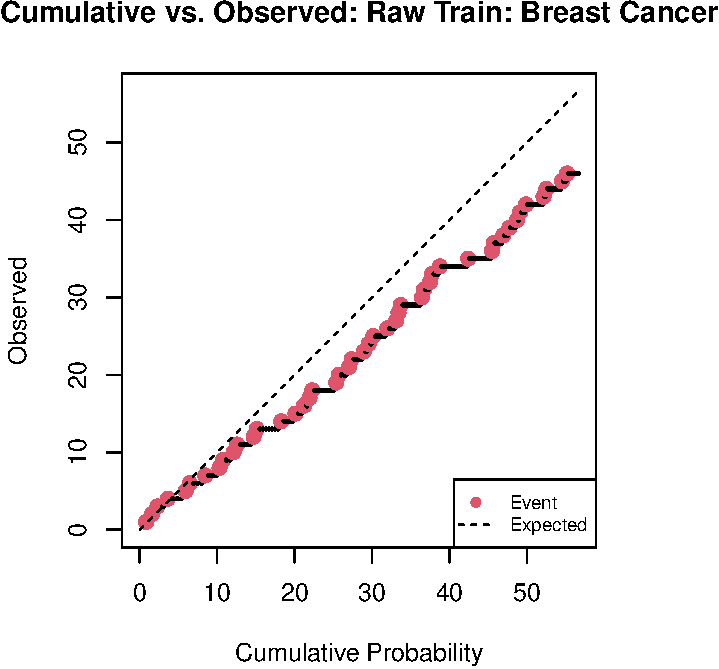
\includegraphics{flchain_files/figure-latex/unnamed-chunk-4-1.pdf}
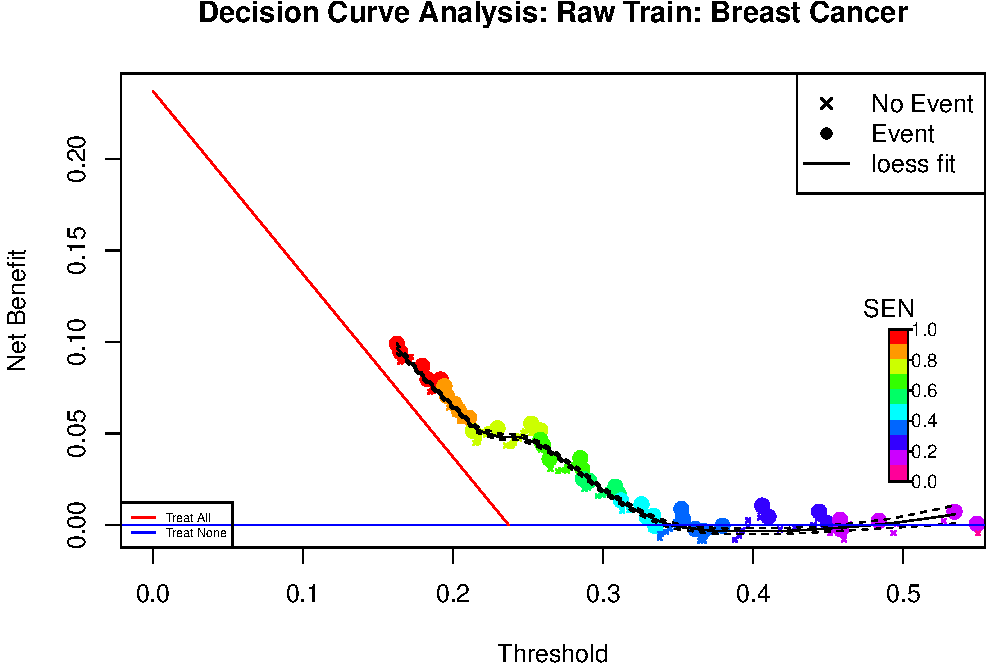
\includegraphics{flchain_files/figure-latex/unnamed-chunk-4-2.pdf}
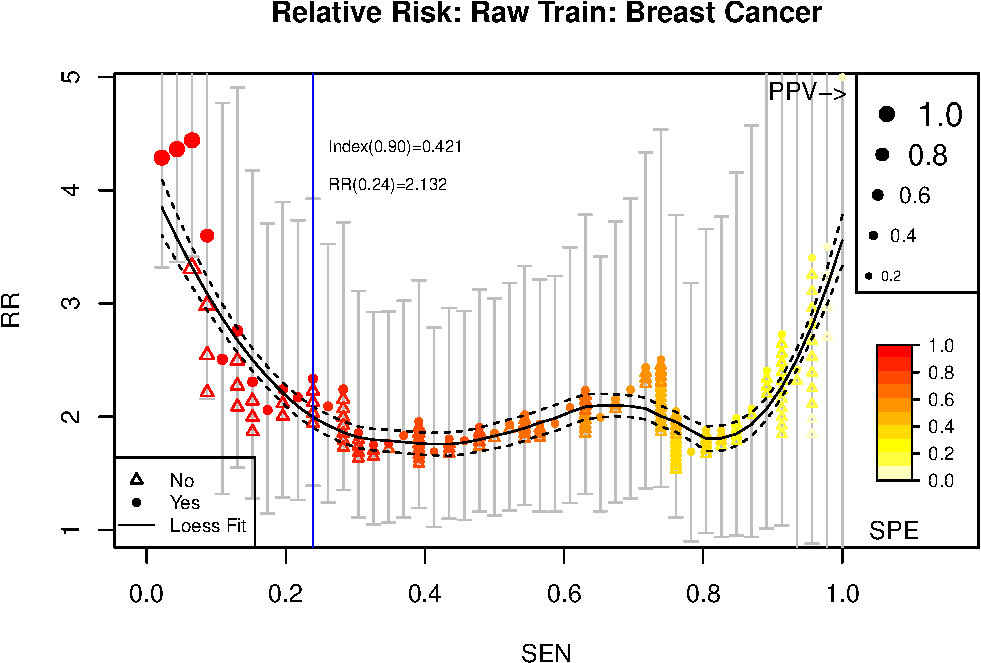
\includegraphics{flchain_files/figure-latex/unnamed-chunk-4-3.pdf}
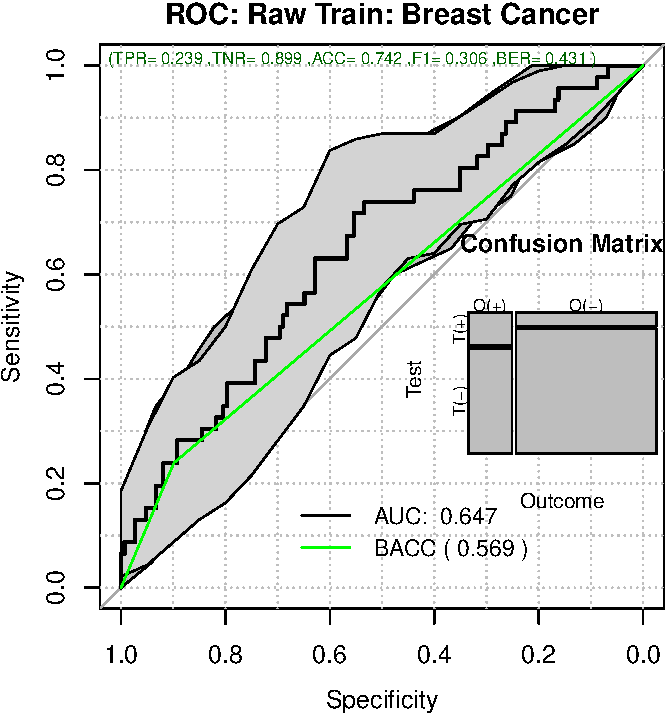
\includegraphics{flchain_files/figure-latex/unnamed-chunk-4-4.pdf}
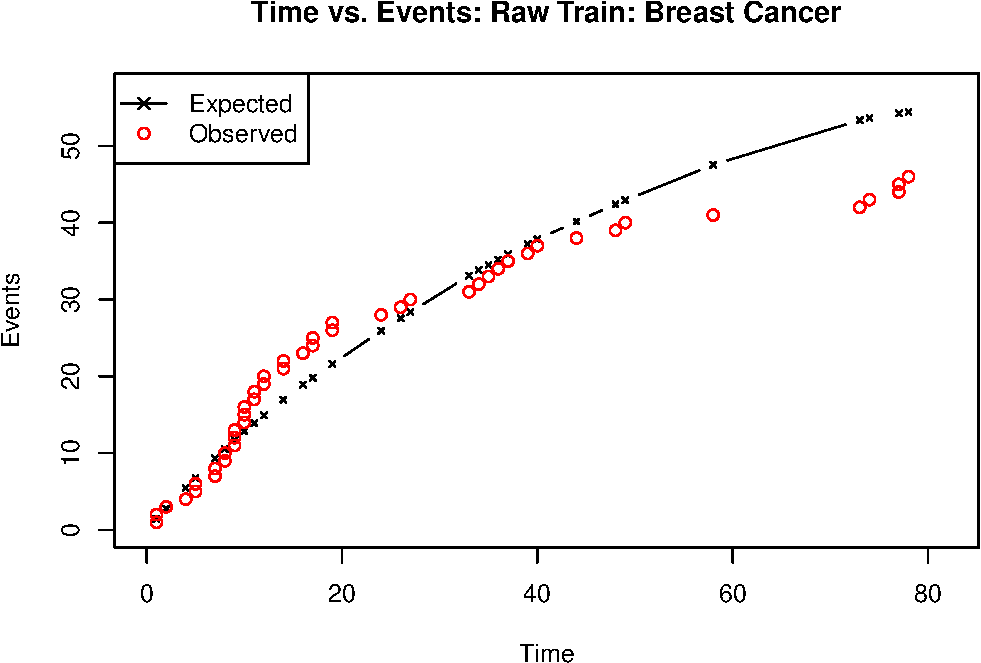
\includegraphics{flchain_files/figure-latex/unnamed-chunk-4-5.pdf}
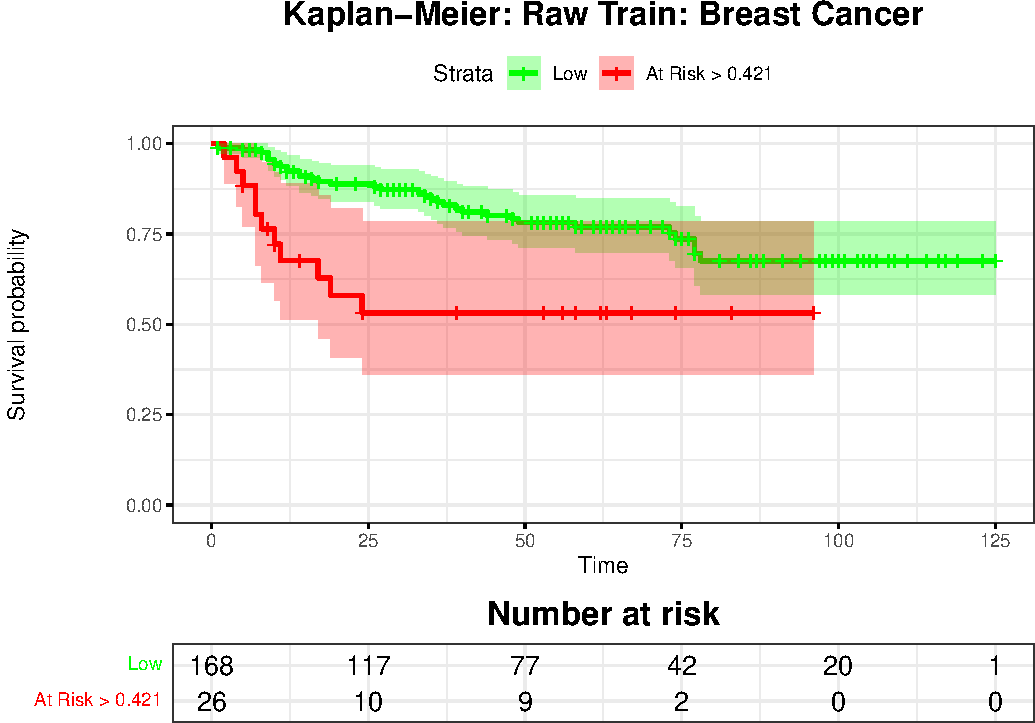
\includegraphics{flchain_files/figure-latex/unnamed-chunk-4-6.pdf}

As we can see the Observed probability as well as the Time vs.~Events
are not calibrated.

\hypertarget{uncalibrated-performance-report}{%
\subsubsection{Uncalibrated Performance
Report}\label{uncalibrated-performance-report}}

\begin{Shaded}
\begin{Highlighting}[]
\NormalTok{pander}\SpecialCharTok{::}\FunctionTok{pander}\NormalTok{(}\FunctionTok{t}\NormalTok{(rrAnalysisTrain}\SpecialCharTok{$}\NormalTok{OERatio),}\AttributeTok{caption=}\StringTok{"O/E Ratio"}\NormalTok{)}
\end{Highlighting}
\end{Shaded}

Quitting from lines 102-115 {[}unnamed-chunk-5{]} (flchain.Rmd) Error in
\texttt{{[}.data.frame}: ! undefined columns selected Backtrace: 1.
pander::pander(t(rrAnalysisTrain\(OERatio), caption = "O/E Ratio")  2. pander:::pander.htest(t(rrAnalysisTrain\)OERatio),
caption = ``O/E Ratio'') 3. pander::pandoc.table(res, caption = caption,
\ldots) 5. pander::pandoc.table.return(\ldots) 7.
base::sapply(1:ncol(t), function(x) is.numeric(t{[}, x{]})) 8.
base::lapply(X = X, FUN = FUN, \ldots) 9. pander (local)
FUN(X{[}{[}i{]}{]}, \ldots) 11. base::\texttt{{[}.data.frame}(t, , x)
Warning messages: 1: In doTryCatch(return(expr), name, parentenv,
handler) : ``quiet'' is not a graphical parameter 2: In
doTryCatch(return(expr), name, parentenv, handler) : ``quiet'' is not a
graphical parameter 3: In doTryCatch(return(expr), name, parentenv,
handler) : ``quiet'' is not a graphical parameter 4: In
doTryCatch(return(expr), name, parentenv, handler) : ``quiet'' is not a
graphical parameter 5: In doTryCatch(return(expr), name, parentenv,
handler) : ``quiet'' is not a graphical parameter 6: In
doTryCatch(return(expr), name, parentenv, handler) : ``quiet'' is not a
graphical parameter 7: In doTryCatch(return(expr), name, parentenv,
handler) : ``quiet'' is not a graphical parameter 8: In
doTryCatch(return(expr), name, parentenv, handler) : ``quiet'' is not a
graphical parameter 9: In doTryCatch(return(expr), name, parentenv,
handler) : ``quiet'' is not a graphical parameter

\begin{Shaded}
\begin{Highlighting}[]
\NormalTok{pander}\SpecialCharTok{::}\FunctionTok{pander}\NormalTok{(}\FunctionTok{t}\NormalTok{(rrAnalysisTrain}\SpecialCharTok{$}\NormalTok{OE95ci),}\AttributeTok{caption=}\StringTok{"O/E Ratio"}\NormalTok{)}
\end{Highlighting}
\end{Shaded}

\begin{longtable}[]{@{}
  >{\centering\arraybackslash}p{(\columnwidth - 6\tabcolsep) * \real{0.1111}}
  >{\centering\arraybackslash}p{(\columnwidth - 6\tabcolsep) * \real{0.1111}}
  >{\centering\arraybackslash}p{(\columnwidth - 6\tabcolsep) * \real{0.0972}}
  >{\centering\arraybackslash}p{(\columnwidth - 6\tabcolsep) * \real{0.1111}}@{}}
\caption{O/E Ratio}\tabularnewline
\toprule\noalign{}
\begin{minipage}[b]{\linewidth}\centering
mean
\end{minipage} & \begin{minipage}[b]{\linewidth}\centering
50\%
\end{minipage} & \begin{minipage}[b]{\linewidth}\centering
2.5\%
\end{minipage} & \begin{minipage}[b]{\linewidth}\centering
97.5\%
\end{minipage} \\
\midrule\noalign{}
\endfirsthead
\toprule\noalign{}
\begin{minipage}[b]{\linewidth}\centering
mean
\end{minipage} & \begin{minipage}[b]{\linewidth}\centering
50\%
\end{minipage} & \begin{minipage}[b]{\linewidth}\centering
2.5\%
\end{minipage} & \begin{minipage}[b]{\linewidth}\centering
97.5\%
\end{minipage} \\
\midrule\noalign{}
\endhead
\bottomrule\noalign{}
\endlastfoot
0.665 & 0.665 & 0.66 & 0.67 \\
\end{longtable}

\begin{Shaded}
\begin{Highlighting}[]
\NormalTok{pander}\SpecialCharTok{::}\FunctionTok{pander}\NormalTok{(}\FunctionTok{t}\NormalTok{(rrAnalysisTrain}\SpecialCharTok{$}\NormalTok{OAcum95ci),}\AttributeTok{caption=}\StringTok{"O/Acum Ratio"}\NormalTok{)}
\end{Highlighting}
\end{Shaded}

\begin{longtable}[]{@{}
  >{\centering\arraybackslash}p{(\columnwidth - 6\tabcolsep) * \real{0.0972}}
  >{\centering\arraybackslash}p{(\columnwidth - 6\tabcolsep) * \real{0.0833}}
  >{\centering\arraybackslash}p{(\columnwidth - 6\tabcolsep) * \real{0.0972}}
  >{\centering\arraybackslash}p{(\columnwidth - 6\tabcolsep) * \real{0.1111}}@{}}
\caption{O/Acum Ratio}\tabularnewline
\toprule\noalign{}
\begin{minipage}[b]{\linewidth}\centering
mean
\end{minipage} & \begin{minipage}[b]{\linewidth}\centering
50\%
\end{minipage} & \begin{minipage}[b]{\linewidth}\centering
2.5\%
\end{minipage} & \begin{minipage}[b]{\linewidth}\centering
97.5\%
\end{minipage} \\
\midrule\noalign{}
\endfirsthead
\toprule\noalign{}
\begin{minipage}[b]{\linewidth}\centering
mean
\end{minipage} & \begin{minipage}[b]{\linewidth}\centering
50\%
\end{minipage} & \begin{minipage}[b]{\linewidth}\centering
2.5\%
\end{minipage} & \begin{minipage}[b]{\linewidth}\centering
97.5\%
\end{minipage} \\
\midrule\noalign{}
\endhead
\bottomrule\noalign{}
\endlastfoot
1.1 & 1.1 & 1.09 & 1.1 \\
\end{longtable}

\begin{Shaded}
\begin{Highlighting}[]
\NormalTok{pander}\SpecialCharTok{::}\FunctionTok{pander}\NormalTok{(}\FunctionTok{t}\NormalTok{(rrAnalysisTrain}\SpecialCharTok{$}\NormalTok{c.index}\SpecialCharTok{$}\NormalTok{cstatCI),}\AttributeTok{caption=}\StringTok{"C. Index"}\NormalTok{)}
\end{Highlighting}
\end{Shaded}

\begin{longtable}[]{@{}
  >{\centering\arraybackslash}p{(\columnwidth - 6\tabcolsep) * \real{0.2083}}
  >{\centering\arraybackslash}p{(\columnwidth - 6\tabcolsep) * \real{0.1250}}
  >{\centering\arraybackslash}p{(\columnwidth - 6\tabcolsep) * \real{0.1111}}
  >{\centering\arraybackslash}p{(\columnwidth - 6\tabcolsep) * \real{0.1111}}@{}}
\caption{C. Index}\tabularnewline
\toprule\noalign{}
\begin{minipage}[b]{\linewidth}\centering
mean.C Index
\end{minipage} & \begin{minipage}[b]{\linewidth}\centering
median
\end{minipage} & \begin{minipage}[b]{\linewidth}\centering
lower
\end{minipage} & \begin{minipage}[b]{\linewidth}\centering
upper
\end{minipage} \\
\midrule\noalign{}
\endfirsthead
\toprule\noalign{}
\begin{minipage}[b]{\linewidth}\centering
mean.C Index
\end{minipage} & \begin{minipage}[b]{\linewidth}\centering
median
\end{minipage} & \begin{minipage}[b]{\linewidth}\centering
lower
\end{minipage} & \begin{minipage}[b]{\linewidth}\centering
upper
\end{minipage} \\
\midrule\noalign{}
\endhead
\bottomrule\noalign{}
\endlastfoot
0.791 & 0.791 & 0.773 & 0.809 \\
\end{longtable}

\begin{Shaded}
\begin{Highlighting}[]
\CommentTok{\#pander::pander(rrAnalysisTrain$c.index,caption="C. Index")}
\NormalTok{pander}\SpecialCharTok{::}\FunctionTok{pander}\NormalTok{(}\FunctionTok{t}\NormalTok{(rrAnalysisTrain}\SpecialCharTok{$}\NormalTok{ROCAnalysis}\SpecialCharTok{$}\NormalTok{aucs),}\AttributeTok{caption=}\StringTok{"ROC AUC"}\NormalTok{)}
\end{Highlighting}
\end{Shaded}

\begin{longtable}[]{@{}
  >{\centering\arraybackslash}p{(\columnwidth - 4\tabcolsep) * \real{0.1111}}
  >{\centering\arraybackslash}p{(\columnwidth - 4\tabcolsep) * \real{0.1111}}
  >{\centering\arraybackslash}p{(\columnwidth - 4\tabcolsep) * \real{0.1111}}@{}}
\caption{ROC AUC}\tabularnewline
\toprule\noalign{}
\begin{minipage}[b]{\linewidth}\centering
est
\end{minipage} & \begin{minipage}[b]{\linewidth}\centering
lower
\end{minipage} & \begin{minipage}[b]{\linewidth}\centering
upper
\end{minipage} \\
\midrule\noalign{}
\endfirsthead
\toprule\noalign{}
\begin{minipage}[b]{\linewidth}\centering
est
\end{minipage} & \begin{minipage}[b]{\linewidth}\centering
lower
\end{minipage} & \begin{minipage}[b]{\linewidth}\centering
upper
\end{minipage} \\
\midrule\noalign{}
\endhead
\bottomrule\noalign{}
\endlastfoot
0.839 & 0.82 & 0.858 \\
\end{longtable}

\begin{Shaded}
\begin{Highlighting}[]
\NormalTok{pander}\SpecialCharTok{::}\FunctionTok{pander}\NormalTok{((rrAnalysisTrain}\SpecialCharTok{$}\NormalTok{ROCAnalysis}\SpecialCharTok{$}\NormalTok{sensitivity),}\AttributeTok{caption=}\StringTok{"Sensitivity"}\NormalTok{)}
\end{Highlighting}
\end{Shaded}

\begin{longtable}[]{@{}
  >{\centering\arraybackslash}p{(\columnwidth - 4\tabcolsep) * \real{0.1111}}
  >{\centering\arraybackslash}p{(\columnwidth - 4\tabcolsep) * \real{0.1111}}
  >{\centering\arraybackslash}p{(\columnwidth - 4\tabcolsep) * \real{0.1111}}@{}}
\caption{Sensitivity}\tabularnewline
\toprule\noalign{}
\begin{minipage}[b]{\linewidth}\centering
est
\end{minipage} & \begin{minipage}[b]{\linewidth}\centering
lower
\end{minipage} & \begin{minipage}[b]{\linewidth}\centering
upper
\end{minipage} \\
\midrule\noalign{}
\endfirsthead
\toprule\noalign{}
\begin{minipage}[b]{\linewidth}\centering
est
\end{minipage} & \begin{minipage}[b]{\linewidth}\centering
lower
\end{minipage} & \begin{minipage}[b]{\linewidth}\centering
upper
\end{minipage} \\
\midrule\noalign{}
\endhead
\bottomrule\noalign{}
\endlastfoot
0.591 & 0.552 & 0.63 \\
\end{longtable}

\begin{Shaded}
\begin{Highlighting}[]
\NormalTok{pander}\SpecialCharTok{::}\FunctionTok{pander}\NormalTok{((rrAnalysisTrain}\SpecialCharTok{$}\NormalTok{ROCAnalysis}\SpecialCharTok{$}\NormalTok{specificity),}\AttributeTok{caption=}\StringTok{"Specificity"}\NormalTok{)}
\end{Highlighting}
\end{Shaded}

\begin{longtable}[]{@{}
  >{\centering\arraybackslash}p{(\columnwidth - 4\tabcolsep) * \real{0.1111}}
  >{\centering\arraybackslash}p{(\columnwidth - 4\tabcolsep) * \real{0.1111}}
  >{\centering\arraybackslash}p{(\columnwidth - 4\tabcolsep) * \real{0.1111}}@{}}
\caption{Specificity}\tabularnewline
\toprule\noalign{}
\begin{minipage}[b]{\linewidth}\centering
est
\end{minipage} & \begin{minipage}[b]{\linewidth}\centering
lower
\end{minipage} & \begin{minipage}[b]{\linewidth}\centering
upper
\end{minipage} \\
\midrule\noalign{}
\endfirsthead
\toprule\noalign{}
\begin{minipage}[b]{\linewidth}\centering
est
\end{minipage} & \begin{minipage}[b]{\linewidth}\centering
lower
\end{minipage} & \begin{minipage}[b]{\linewidth}\centering
upper
\end{minipage} \\
\midrule\noalign{}
\endhead
\bottomrule\noalign{}
\endlastfoot
0.899 & 0.882 & 0.915 \\
\end{longtable}

\begin{Shaded}
\begin{Highlighting}[]
\NormalTok{pander}\SpecialCharTok{::}\FunctionTok{pander}\NormalTok{(}\FunctionTok{t}\NormalTok{(rrAnalysisTrain}\SpecialCharTok{$}\NormalTok{thr\_atP),}\AttributeTok{caption=}\StringTok{"Probability Thresholds"}\NormalTok{)}
\end{Highlighting}
\end{Shaded}

\begin{longtable}[]{@{}
  >{\centering\arraybackslash}p{(\columnwidth - 2\tabcolsep) * \real{0.1111}}
  >{\centering\arraybackslash}p{(\columnwidth - 2\tabcolsep) * \real{0.1111}}@{}}
\caption{Probability Thresholds}\tabularnewline
\toprule\noalign{}
\begin{minipage}[b]{\linewidth}\centering
90\%
\end{minipage} & \begin{minipage}[b]{\linewidth}\centering
80\%
\end{minipage} \\
\midrule\noalign{}
\endfirsthead
\toprule\noalign{}
\begin{minipage}[b]{\linewidth}\centering
90\%
\end{minipage} & \begin{minipage}[b]{\linewidth}\centering
80\%
\end{minipage} \\
\midrule\noalign{}
\endhead
\bottomrule\noalign{}
\endlastfoot
0.321 & 0.22 \\
\end{longtable}

\begin{Shaded}
\begin{Highlighting}[]
\NormalTok{pander}\SpecialCharTok{::}\FunctionTok{pander}\NormalTok{(}\FunctionTok{t}\NormalTok{(rrAnalysisTrain}\SpecialCharTok{$}\NormalTok{RR\_atP),}\AttributeTok{caption=}\StringTok{"Risk Ratio"}\NormalTok{)}
\end{Highlighting}
\end{Shaded}

Quitting from lines 102-115 {[}unnamed-chunk-5{]} (flchain.Rmd) Error in
\texttt{t.default()}: ! argument is not a matrix Backtrace: 1.
pander::pander(t(rrAnalysisTrain\(RR_atP), caption = "Risk Ratio")  3. base::t.default(rrAnalysisTrain\)RR\_atP)

\begin{Shaded}
\begin{Highlighting}[]
\NormalTok{pander}\SpecialCharTok{::}\FunctionTok{pander}\NormalTok{(rrAnalysisTrain}\SpecialCharTok{$}\NormalTok{surdif,}\AttributeTok{caption=}\StringTok{"Logrank test"}\NormalTok{)}
\end{Highlighting}
\end{Shaded}

\begin{longtable}[]{@{}
  >{\centering\arraybackslash}p{(\columnwidth - 10\tabcolsep) * \real{0.1944}}
  >{\centering\arraybackslash}p{(\columnwidth - 10\tabcolsep) * \real{0.0972}}
  >{\centering\arraybackslash}p{(\columnwidth - 10\tabcolsep) * \real{0.1528}}
  >{\centering\arraybackslash}p{(\columnwidth - 10\tabcolsep) * \real{0.1528}}
  >{\centering\arraybackslash}p{(\columnwidth - 10\tabcolsep) * \real{0.1667}}
  >{\centering\arraybackslash}p{(\columnwidth - 10\tabcolsep) * \real{0.1667}}@{}}
\caption{Logrank test Chisq = 772.275840 on 2 degrees of freedom, p =
0.000000}\tabularnewline
\toprule\noalign{}
\begin{minipage}[b]{\linewidth}\centering
~
\end{minipage} & \begin{minipage}[b]{\linewidth}\centering
N
\end{minipage} & \begin{minipage}[b]{\linewidth}\centering
Observed
\end{minipage} & \begin{minipage}[b]{\linewidth}\centering
Expected
\end{minipage} & \begin{minipage}[b]{\linewidth}\centering
(O-E)\^{}2/E
\end{minipage} & \begin{minipage}[b]{\linewidth}\centering
(O-E)\^{}2/V
\end{minipage} \\
\midrule\noalign{}
\endfirsthead
\toprule\noalign{}
\begin{minipage}[b]{\linewidth}\centering
~
\end{minipage} & \begin{minipage}[b]{\linewidth}\centering
N
\end{minipage} & \begin{minipage}[b]{\linewidth}\centering
Observed
\end{minipage} & \begin{minipage}[b]{\linewidth}\centering
Expected
\end{minipage} & \begin{minipage}[b]{\linewidth}\centering
(O-E)\^{}2/E
\end{minipage} & \begin{minipage}[b]{\linewidth}\centering
(O-E)\^{}2/V
\end{minipage} \\
\midrule\noalign{}
\endhead
\bottomrule\noalign{}
\endlastfoot
\textbf{class=0} & 1271 & 176 & 448.2 & 165.34 & 581.5 \\
\textbf{class=1} & 219 & 81 & 67.8 & 2.58 & 2.9 \\
\textbf{class=2} & 510 & 372 & 113.0 & 593.69 & 733.3 \\
\end{longtable}

\hypertarget{cox-calibration}{%
\subsubsection{Cox Calibration}\label{cox-calibration}}

\begin{Shaded}
\begin{Highlighting}[]
\NormalTok{op }\OtherTok{\textless{}{-}} \FunctionTok{par}\NormalTok{(}\AttributeTok{no.readonly =} \ConstantTok{TRUE}\NormalTok{)}


\NormalTok{calprob }\OtherTok{\textless{}{-}} \FunctionTok{CoxRiskCalibration}\NormalTok{(ml,dataFLTrain,}\StringTok{"status"}\NormalTok{,}\StringTok{"time"}\NormalTok{)}
\end{Highlighting}
\end{Shaded}

( 14.74767 , 9389.125 , 1.242363 , 628 , 689.322 )

\begin{Shaded}
\begin{Highlighting}[]
\NormalTok{pander}\SpecialCharTok{::}\FunctionTok{pander}\NormalTok{(}\FunctionTok{c}\NormalTok{(}\AttributeTok{h0=}\NormalTok{calprob}\SpecialCharTok{$}\NormalTok{h0,}
                 \AttributeTok{Gain=}\NormalTok{calprob}\SpecialCharTok{$}\NormalTok{hazardGain,}
                 \AttributeTok{DeltaTime=}\NormalTok{calprob}\SpecialCharTok{$}\NormalTok{timeInterval),}
               \AttributeTok{caption=}\StringTok{"Cox Calibration Parameters"}\NormalTok{)}
\end{Highlighting}
\end{Shaded}

\begin{longtable}[]{@{}
  >{\centering\arraybackslash}p{(\columnwidth - 4\tabcolsep) * \real{0.1111}}
  >{\centering\arraybackslash}p{(\columnwidth - 4\tabcolsep) * \real{0.1111}}
  >{\centering\arraybackslash}p{(\columnwidth - 4\tabcolsep) * \real{0.1667}}@{}}
\toprule\noalign{}
\begin{minipage}[b]{\linewidth}\centering
h0
\end{minipage} & \begin{minipage}[b]{\linewidth}\centering
Gain
\end{minipage} & \begin{minipage}[b]{\linewidth}\centering
DeltaTime
\end{minipage} \\
\midrule\noalign{}
\endhead
\bottomrule\noalign{}
\endlastfoot
0.267 & 0.703 & 14.7 \\
\end{longtable}

\hypertarget{the-rrplot-of-the-calibrated-model}{%
\subsubsection{The RRplot() of the calibrated
model}\label{the-rrplot-of-the-calibrated-model}}

\begin{Shaded}
\begin{Highlighting}[]
\NormalTok{h0 }\OtherTok{\textless{}{-}}\NormalTok{ calprob}\SpecialCharTok{$}\NormalTok{h0}
\NormalTok{timeinterval }\OtherTok{\textless{}{-}}\NormalTok{ calprob}\SpecialCharTok{$}\NormalTok{timeInterval;}

\NormalTok{rdata }\OtherTok{\textless{}{-}} \FunctionTok{cbind}\NormalTok{(dataFLTrain}\SpecialCharTok{$}\NormalTok{status,calprob}\SpecialCharTok{$}\NormalTok{prob)}


\NormalTok{rrAnalysisTrain }\OtherTok{\textless{}{-}} \FunctionTok{RRPlot}\NormalTok{(rdata,}\AttributeTok{atRate=}\FunctionTok{c}\NormalTok{(}\FloatTok{0.90}\NormalTok{,}\FloatTok{0.80}\NormalTok{),}
                     \AttributeTok{timetoEvent=}\NormalTok{dataFLTrain}\SpecialCharTok{$}\NormalTok{time,}
                     \AttributeTok{title=}\StringTok{"Calibrated Train: FLC"}\NormalTok{,}
                     \AttributeTok{ysurvlim=}\FunctionTok{c}\NormalTok{(}\FloatTok{0.00}\NormalTok{,}\FloatTok{1.0}\NormalTok{),}
                     \AttributeTok{riskTimeInterval=}\NormalTok{timeinterval)}
\end{Highlighting}
\end{Shaded}

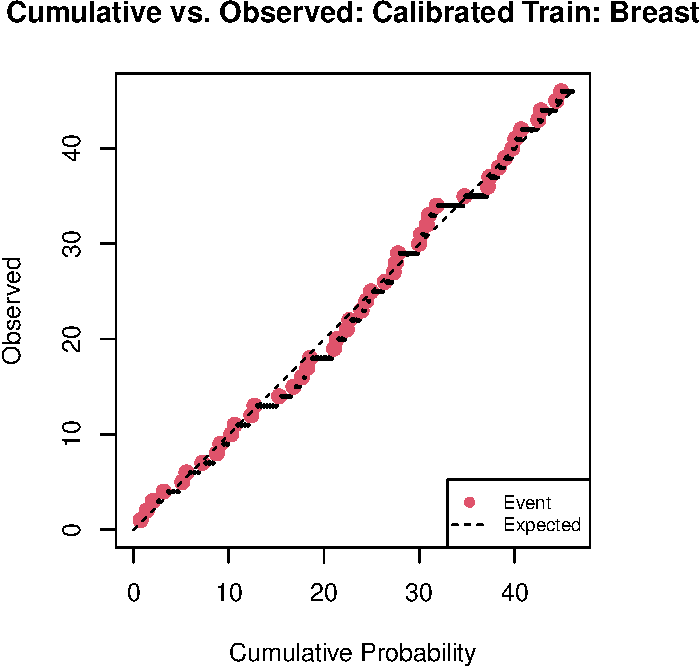
\includegraphics{flchain_files/figure-latex/unnamed-chunk-7-1.pdf}
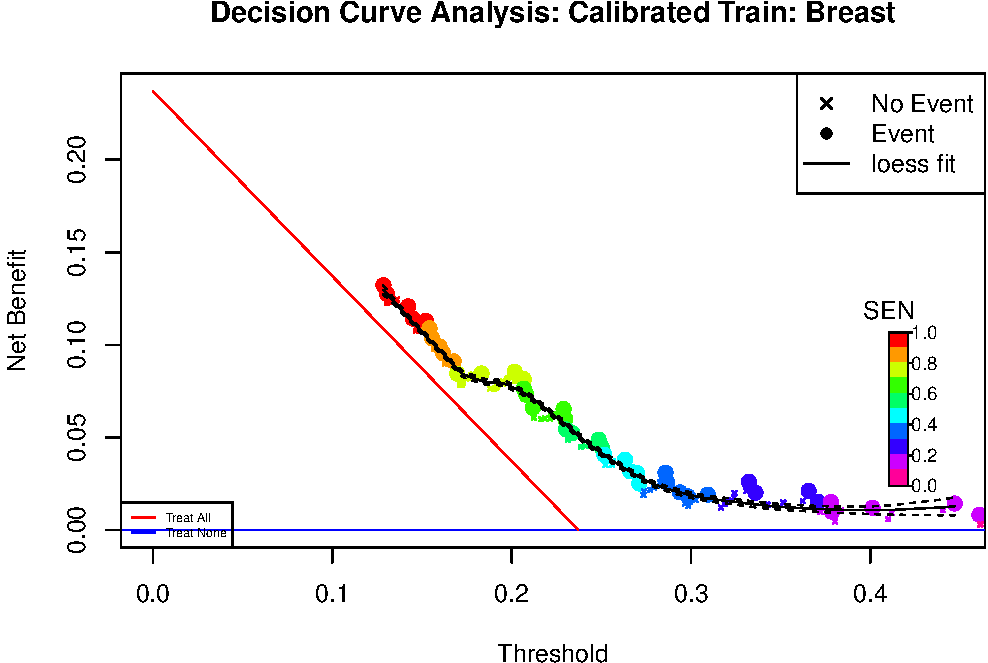
\includegraphics{flchain_files/figure-latex/unnamed-chunk-7-2.pdf}
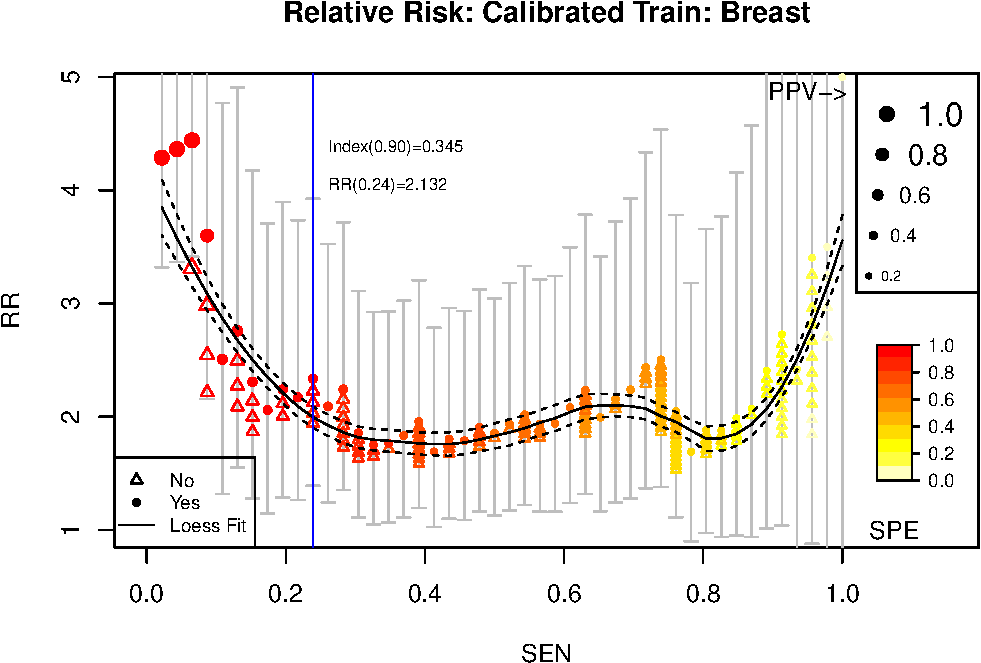
\includegraphics{flchain_files/figure-latex/unnamed-chunk-7-3.pdf}
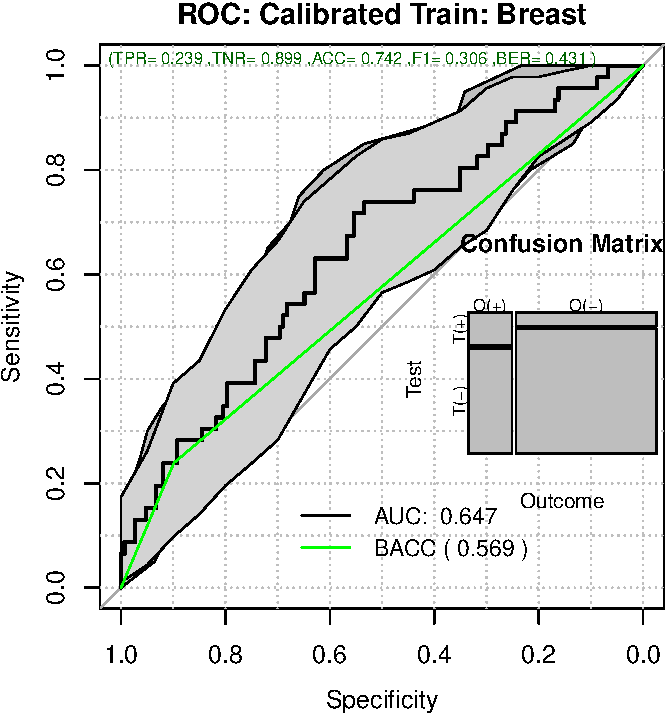
\includegraphics{flchain_files/figure-latex/unnamed-chunk-7-4.pdf}
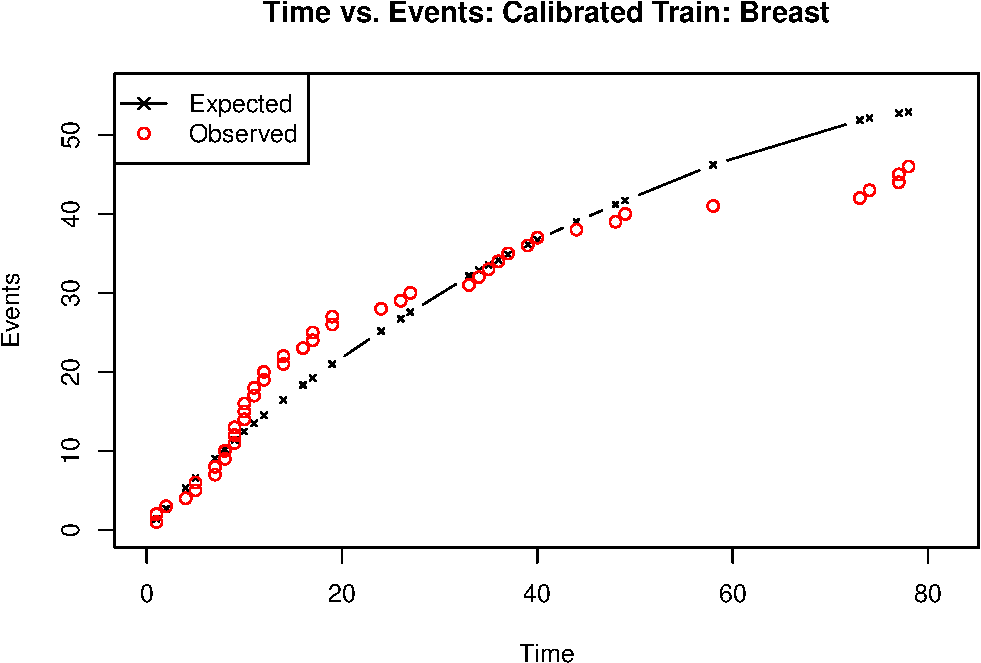
\includegraphics{flchain_files/figure-latex/unnamed-chunk-7-5.pdf}
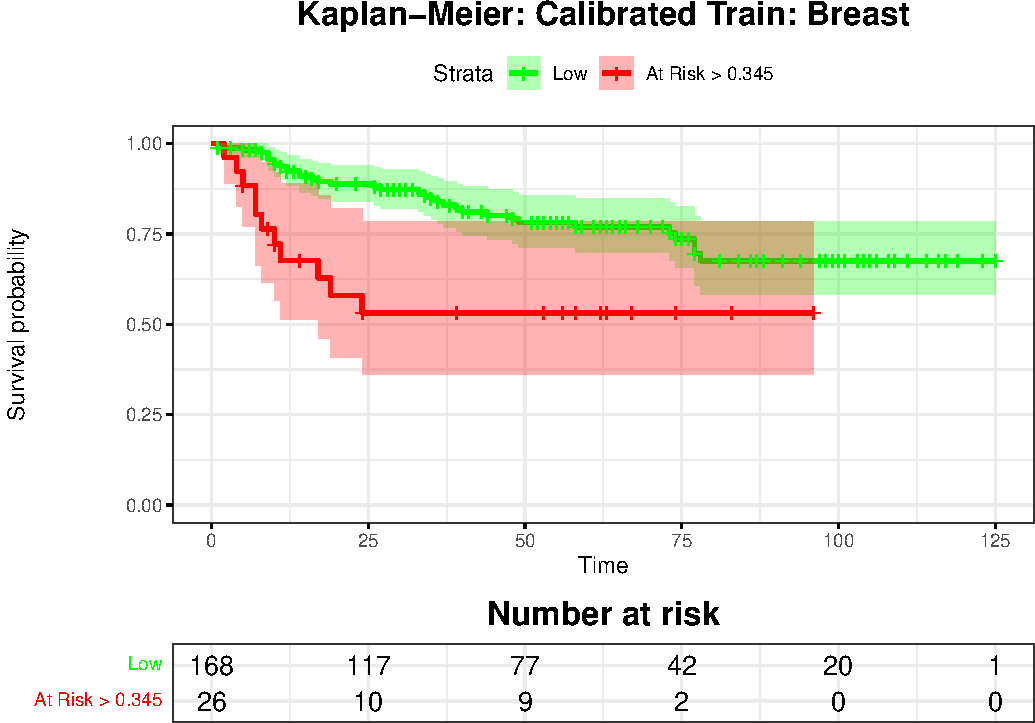
\includegraphics{flchain_files/figure-latex/unnamed-chunk-7-6.pdf}

\hypertarget{calibrated-train-performance}{%
\subsubsection{Calibrated Train
Performance}\label{calibrated-train-performance}}

\begin{Shaded}
\begin{Highlighting}[]
\NormalTok{pander}\SpecialCharTok{::}\FunctionTok{pander}\NormalTok{(}\FunctionTok{t}\NormalTok{(rrAnalysisTrain}\SpecialCharTok{$}\NormalTok{OERatio),}\AttributeTok{caption=}\StringTok{"O/E Ratio"}\NormalTok{)}
\end{Highlighting}
\end{Shaded}

Quitting from lines 153-166 {[}unnamed-chunk-8{]} (flchain.Rmd) Error in
\texttt{{[}.data.frame}: ! undefined columns selected Backtrace: 1.
pander::pander(t(rrAnalysisTrain\(OERatio), caption = "O/E Ratio")  2. pander:::pander.htest(t(rrAnalysisTrain\)OERatio),
caption = ``O/E Ratio'') 3. pander::pandoc.table(res, caption = caption,
\ldots) 5. pander::pandoc.table.return(\ldots) 7.
base::sapply(1:ncol(t), function(x) is.numeric(t{[}, x{]})) 8.
base::lapply(X = X, FUN = FUN, \ldots) 9. pander (local)
FUN(X{[}{[}i{]}{]}, \ldots) 11. base::\texttt{{[}.data.frame}(t, , x)
Warning messages: 1: In doTryCatch(return(expr), name, parentenv,
handler) : ``quiet'' is not a graphical parameter 2: In
doTryCatch(return(expr), name, parentenv, handler) : ``quiet'' is not a
graphical parameter 3: In doTryCatch(return(expr), name, parentenv,
handler) : ``quiet'' is not a graphical parameter 4: In
doTryCatch(return(expr), name, parentenv, handler) : ``quiet'' is not a
graphical parameter 5: In doTryCatch(return(expr), name, parentenv,
handler) : ``quiet'' is not a graphical parameter 6: In
doTryCatch(return(expr), name, parentenv, handler) : ``quiet'' is not a
graphical parameter 7: In doTryCatch(return(expr), name, parentenv,
handler) : ``quiet'' is not a graphical parameter 8: In
doTryCatch(return(expr), name, parentenv, handler) : ``quiet'' is not a
graphical parameter 9: In doTryCatch(return(expr), name, parentenv,
handler) : ``quiet'' is not a graphical parameter

\begin{Shaded}
\begin{Highlighting}[]
\NormalTok{pander}\SpecialCharTok{::}\FunctionTok{pander}\NormalTok{(}\FunctionTok{t}\NormalTok{(rrAnalysisTrain}\SpecialCharTok{$}\NormalTok{OE95ci),}\AttributeTok{caption=}\StringTok{"O/E Ratio"}\NormalTok{)}
\end{Highlighting}
\end{Shaded}

\begin{longtable}[]{@{}
  >{\centering\arraybackslash}p{(\columnwidth - 6\tabcolsep) * \real{0.1111}}
  >{\centering\arraybackslash}p{(\columnwidth - 6\tabcolsep) * \real{0.1111}}
  >{\centering\arraybackslash}p{(\columnwidth - 6\tabcolsep) * \real{0.1111}}
  >{\centering\arraybackslash}p{(\columnwidth - 6\tabcolsep) * \real{0.1111}}@{}}
\caption{O/E Ratio}\tabularnewline
\toprule\noalign{}
\begin{minipage}[b]{\linewidth}\centering
mean
\end{minipage} & \begin{minipage}[b]{\linewidth}\centering
50\%
\end{minipage} & \begin{minipage}[b]{\linewidth}\centering
2.5\%
\end{minipage} & \begin{minipage}[b]{\linewidth}\centering
97.5\%
\end{minipage} \\
\midrule\noalign{}
\endfirsthead
\toprule\noalign{}
\begin{minipage}[b]{\linewidth}\centering
mean
\end{minipage} & \begin{minipage}[b]{\linewidth}\centering
50\%
\end{minipage} & \begin{minipage}[b]{\linewidth}\centering
2.5\%
\end{minipage} & \begin{minipage}[b]{\linewidth}\centering
97.5\%
\end{minipage} \\
\midrule\noalign{}
\endhead
\bottomrule\noalign{}
\endlastfoot
0.998 & 0.998 & 0.993 & 1 \\
\end{longtable}

\begin{Shaded}
\begin{Highlighting}[]
\NormalTok{pander}\SpecialCharTok{::}\FunctionTok{pander}\NormalTok{(}\FunctionTok{t}\NormalTok{(rrAnalysisTrain}\SpecialCharTok{$}\NormalTok{OAcum95ci),}\AttributeTok{caption=}\StringTok{"O/Acum Ratio"}\NormalTok{)}
\end{Highlighting}
\end{Shaded}

\begin{longtable}[]{@{}
  >{\centering\arraybackslash}p{(\columnwidth - 6\tabcolsep) * \real{0.0972}}
  >{\centering\arraybackslash}p{(\columnwidth - 6\tabcolsep) * \real{0.0972}}
  >{\centering\arraybackslash}p{(\columnwidth - 6\tabcolsep) * \real{0.0972}}
  >{\centering\arraybackslash}p{(\columnwidth - 6\tabcolsep) * \real{0.1111}}@{}}
\caption{O/Acum Ratio}\tabularnewline
\toprule\noalign{}
\begin{minipage}[b]{\linewidth}\centering
mean
\end{minipage} & \begin{minipage}[b]{\linewidth}\centering
50\%
\end{minipage} & \begin{minipage}[b]{\linewidth}\centering
2.5\%
\end{minipage} & \begin{minipage}[b]{\linewidth}\centering
97.5\%
\end{minipage} \\
\midrule\noalign{}
\endfirsthead
\toprule\noalign{}
\begin{minipage}[b]{\linewidth}\centering
mean
\end{minipage} & \begin{minipage}[b]{\linewidth}\centering
50\%
\end{minipage} & \begin{minipage}[b]{\linewidth}\centering
2.5\%
\end{minipage} & \begin{minipage}[b]{\linewidth}\centering
97.5\%
\end{minipage} \\
\midrule\noalign{}
\endhead
\bottomrule\noalign{}
\endlastfoot
1.04 & 1.04 & 1.04 & 1.05 \\
\end{longtable}

\begin{Shaded}
\begin{Highlighting}[]
\NormalTok{pander}\SpecialCharTok{::}\FunctionTok{pander}\NormalTok{(}\FunctionTok{t}\NormalTok{(rrAnalysisTrain}\SpecialCharTok{$}\NormalTok{c.index}\SpecialCharTok{$}\NormalTok{cstatCI),}\AttributeTok{caption=}\StringTok{"C. Index"}\NormalTok{)}
\end{Highlighting}
\end{Shaded}

\begin{longtable}[]{@{}
  >{\centering\arraybackslash}p{(\columnwidth - 6\tabcolsep) * \real{0.2083}}
  >{\centering\arraybackslash}p{(\columnwidth - 6\tabcolsep) * \real{0.1250}}
  >{\centering\arraybackslash}p{(\columnwidth - 6\tabcolsep) * \real{0.1111}}
  >{\centering\arraybackslash}p{(\columnwidth - 6\tabcolsep) * \real{0.1111}}@{}}
\caption{C. Index}\tabularnewline
\toprule\noalign{}
\begin{minipage}[b]{\linewidth}\centering
mean.C Index
\end{minipage} & \begin{minipage}[b]{\linewidth}\centering
median
\end{minipage} & \begin{minipage}[b]{\linewidth}\centering
lower
\end{minipage} & \begin{minipage}[b]{\linewidth}\centering
upper
\end{minipage} \\
\midrule\noalign{}
\endfirsthead
\toprule\noalign{}
\begin{minipage}[b]{\linewidth}\centering
mean.C Index
\end{minipage} & \begin{minipage}[b]{\linewidth}\centering
median
\end{minipage} & \begin{minipage}[b]{\linewidth}\centering
lower
\end{minipage} & \begin{minipage}[b]{\linewidth}\centering
upper
\end{minipage} \\
\midrule\noalign{}
\endhead
\bottomrule\noalign{}
\endlastfoot
0.791 & 0.791 & 0.773 & 0.808 \\
\end{longtable}

\begin{Shaded}
\begin{Highlighting}[]
\CommentTok{\#pander::pander(rrAnalysisTrain$c.index,caption="C. Index")}
\NormalTok{pander}\SpecialCharTok{::}\FunctionTok{pander}\NormalTok{(}\FunctionTok{t}\NormalTok{(rrAnalysisTrain}\SpecialCharTok{$}\NormalTok{ROCAnalysis}\SpecialCharTok{$}\NormalTok{aucs),}\AttributeTok{caption=}\StringTok{"ROC AUC"}\NormalTok{)}
\end{Highlighting}
\end{Shaded}

\begin{longtable}[]{@{}
  >{\centering\arraybackslash}p{(\columnwidth - 4\tabcolsep) * \real{0.1111}}
  >{\centering\arraybackslash}p{(\columnwidth - 4\tabcolsep) * \real{0.1111}}
  >{\centering\arraybackslash}p{(\columnwidth - 4\tabcolsep) * \real{0.1111}}@{}}
\caption{ROC AUC}\tabularnewline
\toprule\noalign{}
\begin{minipage}[b]{\linewidth}\centering
est
\end{minipage} & \begin{minipage}[b]{\linewidth}\centering
lower
\end{minipage} & \begin{minipage}[b]{\linewidth}\centering
upper
\end{minipage} \\
\midrule\noalign{}
\endfirsthead
\toprule\noalign{}
\begin{minipage}[b]{\linewidth}\centering
est
\end{minipage} & \begin{minipage}[b]{\linewidth}\centering
lower
\end{minipage} & \begin{minipage}[b]{\linewidth}\centering
upper
\end{minipage} \\
\midrule\noalign{}
\endhead
\bottomrule\noalign{}
\endlastfoot
0.839 & 0.82 & 0.858 \\
\end{longtable}

\begin{Shaded}
\begin{Highlighting}[]
\NormalTok{pander}\SpecialCharTok{::}\FunctionTok{pander}\NormalTok{((rrAnalysisTrain}\SpecialCharTok{$}\NormalTok{ROCAnalysis}\SpecialCharTok{$}\NormalTok{sensitivity),}\AttributeTok{caption=}\StringTok{"Sensitivity"}\NormalTok{)}
\end{Highlighting}
\end{Shaded}

\begin{longtable}[]{@{}
  >{\centering\arraybackslash}p{(\columnwidth - 4\tabcolsep) * \real{0.1111}}
  >{\centering\arraybackslash}p{(\columnwidth - 4\tabcolsep) * \real{0.1111}}
  >{\centering\arraybackslash}p{(\columnwidth - 4\tabcolsep) * \real{0.1111}}@{}}
\caption{Sensitivity}\tabularnewline
\toprule\noalign{}
\begin{minipage}[b]{\linewidth}\centering
est
\end{minipage} & \begin{minipage}[b]{\linewidth}\centering
lower
\end{minipage} & \begin{minipage}[b]{\linewidth}\centering
upper
\end{minipage} \\
\midrule\noalign{}
\endfirsthead
\toprule\noalign{}
\begin{minipage}[b]{\linewidth}\centering
est
\end{minipage} & \begin{minipage}[b]{\linewidth}\centering
lower
\end{minipage} & \begin{minipage}[b]{\linewidth}\centering
upper
\end{minipage} \\
\midrule\noalign{}
\endhead
\bottomrule\noalign{}
\endlastfoot
0.591 & 0.552 & 0.63 \\
\end{longtable}

\begin{Shaded}
\begin{Highlighting}[]
\NormalTok{pander}\SpecialCharTok{::}\FunctionTok{pander}\NormalTok{((rrAnalysisTrain}\SpecialCharTok{$}\NormalTok{ROCAnalysis}\SpecialCharTok{$}\NormalTok{specificity),}\AttributeTok{caption=}\StringTok{"Specificity"}\NormalTok{)}
\end{Highlighting}
\end{Shaded}

\begin{longtable}[]{@{}
  >{\centering\arraybackslash}p{(\columnwidth - 4\tabcolsep) * \real{0.1111}}
  >{\centering\arraybackslash}p{(\columnwidth - 4\tabcolsep) * \real{0.1111}}
  >{\centering\arraybackslash}p{(\columnwidth - 4\tabcolsep) * \real{0.1111}}@{}}
\caption{Specificity}\tabularnewline
\toprule\noalign{}
\begin{minipage}[b]{\linewidth}\centering
est
\end{minipage} & \begin{minipage}[b]{\linewidth}\centering
lower
\end{minipage} & \begin{minipage}[b]{\linewidth}\centering
upper
\end{minipage} \\
\midrule\noalign{}
\endfirsthead
\toprule\noalign{}
\begin{minipage}[b]{\linewidth}\centering
est
\end{minipage} & \begin{minipage}[b]{\linewidth}\centering
lower
\end{minipage} & \begin{minipage}[b]{\linewidth}\centering
upper
\end{minipage} \\
\midrule\noalign{}
\endhead
\bottomrule\noalign{}
\endlastfoot
0.899 & 0.882 & 0.915 \\
\end{longtable}

\begin{Shaded}
\begin{Highlighting}[]
\NormalTok{pander}\SpecialCharTok{::}\FunctionTok{pander}\NormalTok{(}\FunctionTok{t}\NormalTok{(rrAnalysisTrain}\SpecialCharTok{$}\NormalTok{thr\_atP),}\AttributeTok{caption=}\StringTok{"Probability Thresholds"}\NormalTok{)}
\end{Highlighting}
\end{Shaded}

\begin{longtable}[]{@{}
  >{\centering\arraybackslash}p{(\columnwidth - 2\tabcolsep) * \real{0.1111}}
  >{\centering\arraybackslash}p{(\columnwidth - 2\tabcolsep) * \real{0.1111}}@{}}
\caption{Probability Thresholds}\tabularnewline
\toprule\noalign{}
\begin{minipage}[b]{\linewidth}\centering
90\%
\end{minipage} & \begin{minipage}[b]{\linewidth}\centering
80\%
\end{minipage} \\
\midrule\noalign{}
\endfirsthead
\toprule\noalign{}
\begin{minipage}[b]{\linewidth}\centering
90\%
\end{minipage} & \begin{minipage}[b]{\linewidth}\centering
80\%
\end{minipage} \\
\midrule\noalign{}
\endhead
\bottomrule\noalign{}
\endlastfoot
0.471 & 0.336 \\
\end{longtable}

\begin{Shaded}
\begin{Highlighting}[]
\NormalTok{pander}\SpecialCharTok{::}\FunctionTok{pander}\NormalTok{(}\FunctionTok{t}\NormalTok{(rrAnalysisTrain}\SpecialCharTok{$}\NormalTok{RR\_atP),}\AttributeTok{caption=}\StringTok{"Risk Ratio"}\NormalTok{)}
\end{Highlighting}
\end{Shaded}

Quitting from lines 153-166 {[}unnamed-chunk-8{]} (flchain.Rmd) Error in
\texttt{t.default()}: ! argument is not a matrix Backtrace: 1.
pander::pander(t(rrAnalysisTrain\(RR_atP), caption = "Risk Ratio")  3. base::t.default(rrAnalysisTrain\)RR\_atP)

\begin{Shaded}
\begin{Highlighting}[]
\NormalTok{pander}\SpecialCharTok{::}\FunctionTok{pander}\NormalTok{(rrAnalysisTrain}\SpecialCharTok{$}\NormalTok{surdif,}\AttributeTok{caption=}\StringTok{"Logrank test"}\NormalTok{)}
\end{Highlighting}
\end{Shaded}

\begin{longtable}[]{@{}
  >{\centering\arraybackslash}p{(\columnwidth - 10\tabcolsep) * \real{0.1944}}
  >{\centering\arraybackslash}p{(\columnwidth - 10\tabcolsep) * \real{0.0972}}
  >{\centering\arraybackslash}p{(\columnwidth - 10\tabcolsep) * \real{0.1528}}
  >{\centering\arraybackslash}p{(\columnwidth - 10\tabcolsep) * \real{0.1528}}
  >{\centering\arraybackslash}p{(\columnwidth - 10\tabcolsep) * \real{0.1667}}
  >{\centering\arraybackslash}p{(\columnwidth - 10\tabcolsep) * \real{0.1667}}@{}}
\caption{Logrank test Chisq = 772.275840 on 2 degrees of freedom, p =
0.000000}\tabularnewline
\toprule\noalign{}
\begin{minipage}[b]{\linewidth}\centering
~
\end{minipage} & \begin{minipage}[b]{\linewidth}\centering
N
\end{minipage} & \begin{minipage}[b]{\linewidth}\centering
Observed
\end{minipage} & \begin{minipage}[b]{\linewidth}\centering
Expected
\end{minipage} & \begin{minipage}[b]{\linewidth}\centering
(O-E)\^{}2/E
\end{minipage} & \begin{minipage}[b]{\linewidth}\centering
(O-E)\^{}2/V
\end{minipage} \\
\midrule\noalign{}
\endfirsthead
\toprule\noalign{}
\begin{minipage}[b]{\linewidth}\centering
~
\end{minipage} & \begin{minipage}[b]{\linewidth}\centering
N
\end{minipage} & \begin{minipage}[b]{\linewidth}\centering
Observed
\end{minipage} & \begin{minipage}[b]{\linewidth}\centering
Expected
\end{minipage} & \begin{minipage}[b]{\linewidth}\centering
(O-E)\^{}2/E
\end{minipage} & \begin{minipage}[b]{\linewidth}\centering
(O-E)\^{}2/V
\end{minipage} \\
\midrule\noalign{}
\endhead
\bottomrule\noalign{}
\endlastfoot
\textbf{class=0} & 1271 & 176 & 448.2 & 165.34 & 581.5 \\
\textbf{class=1} & 219 & 81 & 67.8 & 2.58 & 2.9 \\
\textbf{class=2} & 510 & 372 & 113.0 & 593.69 & 733.3 \\
\end{longtable}

\hypertarget{performance-on-the-test-data-set}{%
\subsection{Performance on the test data
set}\label{performance-on-the-test-data-set}}

\begin{Shaded}
\begin{Highlighting}[]
\NormalTok{index }\OtherTok{\textless{}{-}} \FunctionTok{predict}\NormalTok{(ml,dataFLTest)}
\NormalTok{pp }\OtherTok{\textless{}{-}} \FunctionTok{predictionStats\_binary}\NormalTok{(}\FunctionTok{cbind}\NormalTok{(dataFLTest}\SpecialCharTok{$}\NormalTok{status,index),}\AttributeTok{plotname=}\StringTok{"FLC"}\NormalTok{)}
\end{Highlighting}
\end{Shaded}

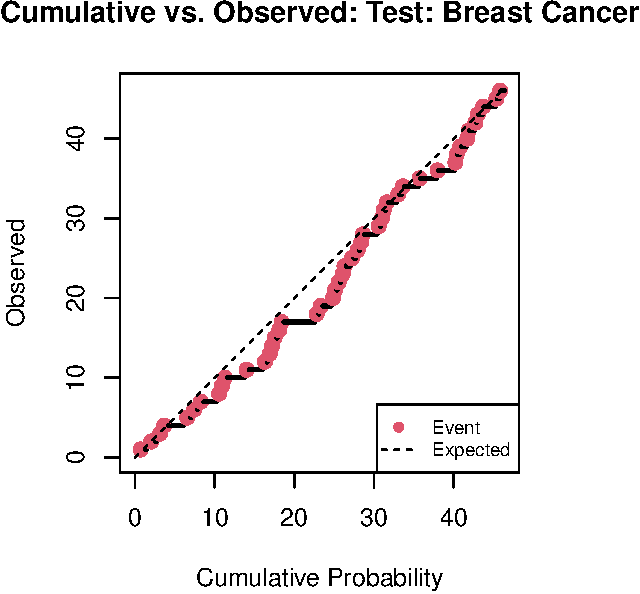
\includegraphics{flchain_files/figure-latex/unnamed-chunk-9-1.pdf}

\begin{Shaded}
\begin{Highlighting}[]
\FunctionTok{par}\NormalTok{(op)}


\NormalTok{prob }\OtherTok{\textless{}{-}} \FunctionTok{ppoisGzero}\NormalTok{(index,h0)}
\NormalTok{rdata }\OtherTok{\textless{}{-}} \FunctionTok{cbind}\NormalTok{(dataFLTest}\SpecialCharTok{$}\NormalTok{status,prob)}
\NormalTok{rrAnalysis }\OtherTok{\textless{}{-}} \FunctionTok{RRPlot}\NormalTok{(rdata,}\AttributeTok{atThr=}\NormalTok{rrAnalysisTrain}\SpecialCharTok{$}\NormalTok{thr\_atP,}
                     \AttributeTok{timetoEvent=}\NormalTok{dataFLTest}\SpecialCharTok{$}\NormalTok{time,}
                     \AttributeTok{title=}\StringTok{"Test: FLC"}\NormalTok{,}
                     \AttributeTok{ysurvlim=}\FunctionTok{c}\NormalTok{(}\FloatTok{0.00}\NormalTok{,}\FloatTok{1.0}\NormalTok{),}
                     \AttributeTok{riskTimeInterval=}\NormalTok{timeinterval)}
\end{Highlighting}
\end{Shaded}

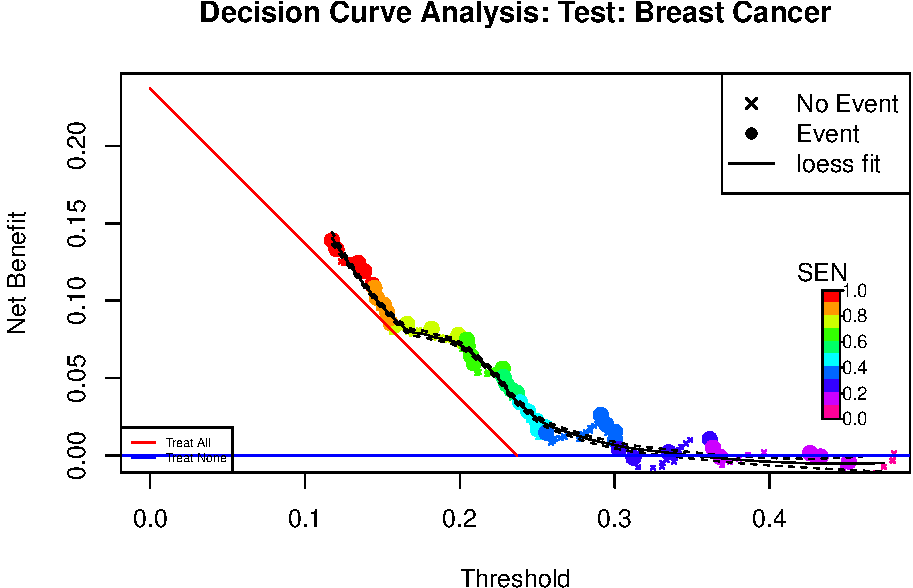
\includegraphics{flchain_files/figure-latex/unnamed-chunk-9-2.pdf}
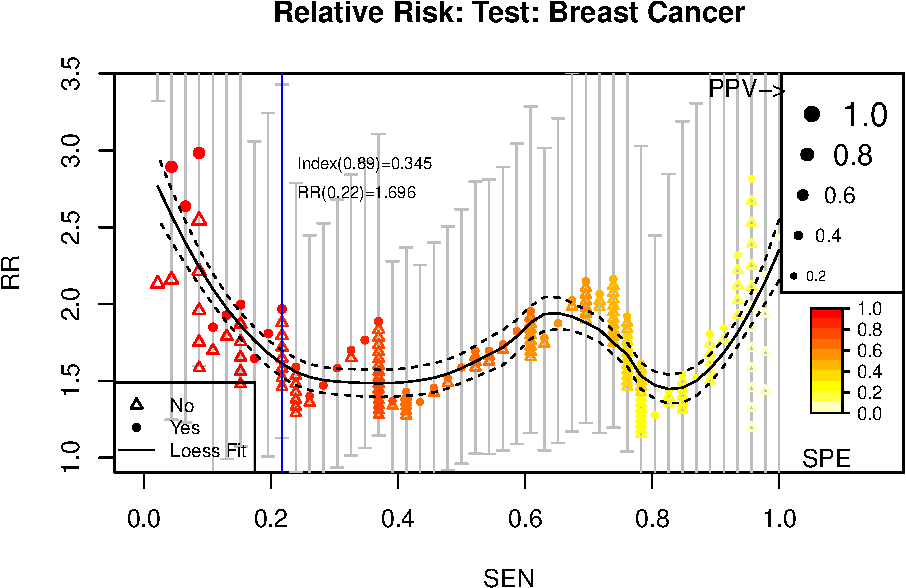
\includegraphics{flchain_files/figure-latex/unnamed-chunk-9-3.pdf}
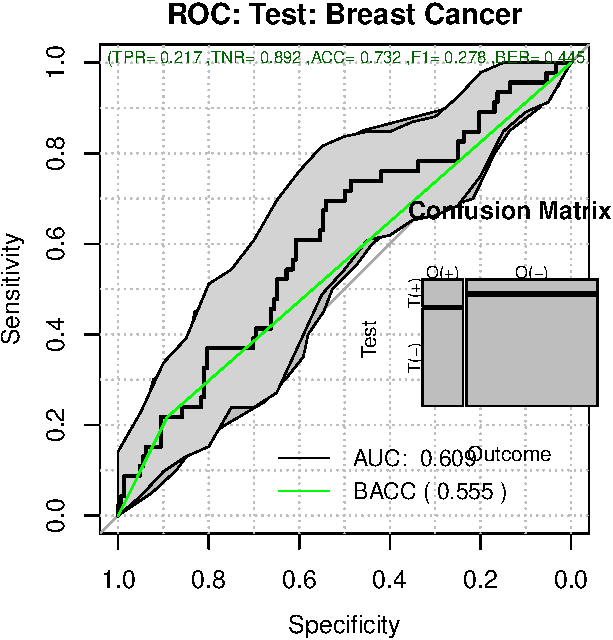
\includegraphics{flchain_files/figure-latex/unnamed-chunk-9-4.pdf}
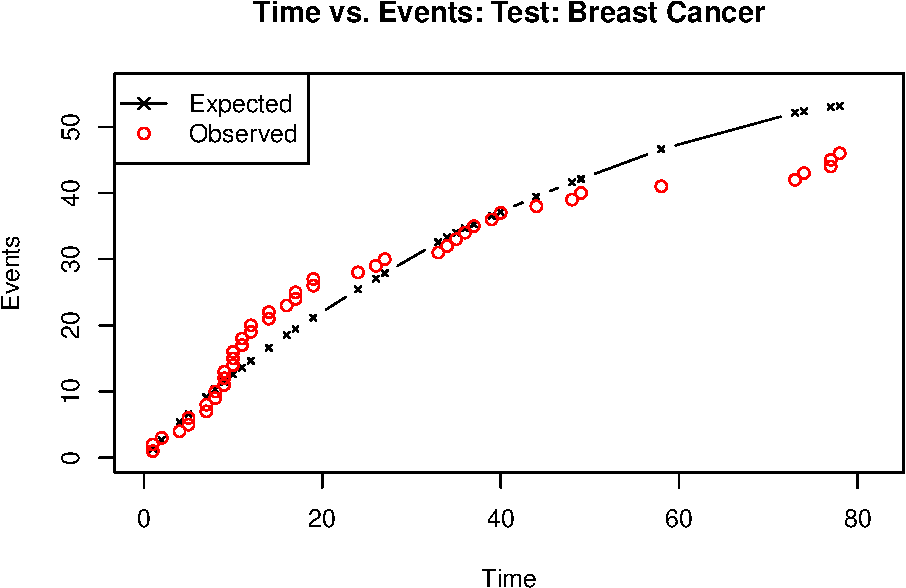
\includegraphics{flchain_files/figure-latex/unnamed-chunk-9-5.pdf}
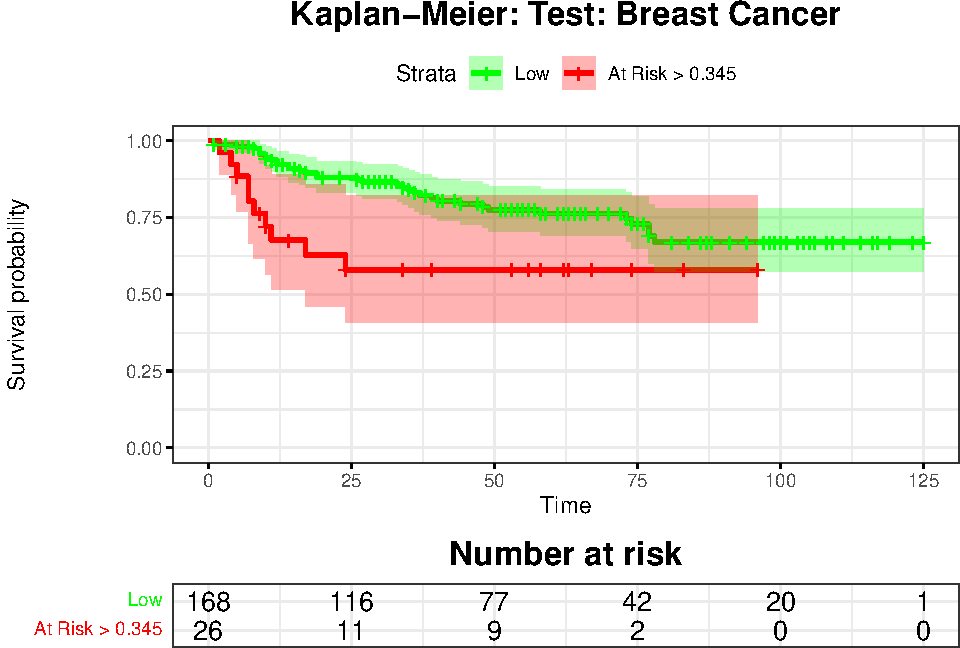
\includegraphics{flchain_files/figure-latex/unnamed-chunk-9-6.pdf}
\includegraphics{flchain_files/figure-latex/unnamed-chunk-9-7.pdf}

\begin{Shaded}
\begin{Highlighting}[]
\FunctionTok{par}\NormalTok{(op)}
\end{Highlighting}
\end{Shaded}

\hypertarget{external-data-report}{%
\subsubsection{External Data Report}\label{external-data-report}}

\begin{Shaded}
\begin{Highlighting}[]
\NormalTok{pander}\SpecialCharTok{::}\FunctionTok{pander}\NormalTok{(}\FunctionTok{t}\NormalTok{(rrAnalysis}\SpecialCharTok{$}\NormalTok{OERatio),}\AttributeTok{caption=}\StringTok{"O/E Ratio"}\NormalTok{)}
\end{Highlighting}
\end{Shaded}

Quitting from lines 193-205 {[}unnamed-chunk-10{]} (flchain.Rmd) Error
in \texttt{{[}.data.frame}: ! undefined columns selected Backtrace: 1.
pander::pander(t(rrAnalysis\(OERatio), caption = "O/E Ratio")  2. pander:::pander.htest(t(rrAnalysis\)OERatio),
caption = ``O/E Ratio'') 3. pander::pandoc.table(res, caption = caption,
\ldots) 5. pander::pandoc.table.return(\ldots) 7.
base::sapply(1:ncol(t), function(x) is.numeric(t{[}, x{]})) 8.
base::lapply(X = X, FUN = FUN, \ldots) 9. pander (local)
FUN(X{[}{[}i{]}{]}, \ldots) 11. base::\texttt{{[}.data.frame}(t, , x)
There were 18 warnings (use warnings() to see them)

\begin{Shaded}
\begin{Highlighting}[]
\NormalTok{pander}\SpecialCharTok{::}\FunctionTok{pander}\NormalTok{(}\FunctionTok{t}\NormalTok{(rrAnalysis}\SpecialCharTok{$}\NormalTok{OE95ci),}\AttributeTok{caption=}\StringTok{"O/E Ratio"}\NormalTok{)}
\end{Highlighting}
\end{Shaded}

\begin{longtable}[]{@{}
  >{\centering\arraybackslash}p{(\columnwidth - 6\tabcolsep) * \real{0.1111}}
  >{\centering\arraybackslash}p{(\columnwidth - 6\tabcolsep) * \real{0.1111}}
  >{\centering\arraybackslash}p{(\columnwidth - 6\tabcolsep) * \real{0.1111}}
  >{\centering\arraybackslash}p{(\columnwidth - 6\tabcolsep) * \real{0.1111}}@{}}
\caption{O/E Ratio}\tabularnewline
\toprule\noalign{}
\begin{minipage}[b]{\linewidth}\centering
mean
\end{minipage} & \begin{minipage}[b]{\linewidth}\centering
50\%
\end{minipage} & \begin{minipage}[b]{\linewidth}\centering
2.5\%
\end{minipage} & \begin{minipage}[b]{\linewidth}\centering
97.5\%
\end{minipage} \\
\midrule\noalign{}
\endfirsthead
\toprule\noalign{}
\begin{minipage}[b]{\linewidth}\centering
mean
\end{minipage} & \begin{minipage}[b]{\linewidth}\centering
50\%
\end{minipage} & \begin{minipage}[b]{\linewidth}\centering
2.5\%
\end{minipage} & \begin{minipage}[b]{\linewidth}\centering
97.5\%
\end{minipage} \\
\midrule\noalign{}
\endhead
\bottomrule\noalign{}
\endlastfoot
0.897 & 0.896 & 0.892 & 0.901 \\
\end{longtable}

\begin{Shaded}
\begin{Highlighting}[]
\NormalTok{pander}\SpecialCharTok{::}\FunctionTok{pander}\NormalTok{(}\FunctionTok{t}\NormalTok{(rrAnalysis}\SpecialCharTok{$}\NormalTok{OAcum95ci),}\AttributeTok{caption=}\StringTok{"O/Acum Ratio"}\NormalTok{)}
\end{Highlighting}
\end{Shaded}

\begin{longtable}[]{@{}
  >{\centering\arraybackslash}p{(\columnwidth - 6\tabcolsep) * \real{0.1111}}
  >{\centering\arraybackslash}p{(\columnwidth - 6\tabcolsep) * \real{0.1111}}
  >{\centering\arraybackslash}p{(\columnwidth - 6\tabcolsep) * \real{0.1111}}
  >{\centering\arraybackslash}p{(\columnwidth - 6\tabcolsep) * \real{0.1111}}@{}}
\caption{O/Acum Ratio}\tabularnewline
\toprule\noalign{}
\begin{minipage}[b]{\linewidth}\centering
mean
\end{minipage} & \begin{minipage}[b]{\linewidth}\centering
50\%
\end{minipage} & \begin{minipage}[b]{\linewidth}\centering
2.5\%
\end{minipage} & \begin{minipage}[b]{\linewidth}\centering
97.5\%
\end{minipage} \\
\midrule\noalign{}
\endfirsthead
\toprule\noalign{}
\begin{minipage}[b]{\linewidth}\centering
mean
\end{minipage} & \begin{minipage}[b]{\linewidth}\centering
50\%
\end{minipage} & \begin{minipage}[b]{\linewidth}\centering
2.5\%
\end{minipage} & \begin{minipage}[b]{\linewidth}\centering
97.5\%
\end{minipage} \\
\midrule\noalign{}
\endhead
\bottomrule\noalign{}
\endlastfoot
0.991 & 0.991 & 0.991 & 0.992 \\
\end{longtable}

\begin{Shaded}
\begin{Highlighting}[]
\NormalTok{pander}\SpecialCharTok{::}\FunctionTok{pander}\NormalTok{(}\FunctionTok{t}\NormalTok{(rrAnalysis}\SpecialCharTok{$}\NormalTok{c.index}\SpecialCharTok{$}\NormalTok{cstatCI),}\AttributeTok{caption=}\StringTok{"C. Index"}\NormalTok{)}
\end{Highlighting}
\end{Shaded}

\begin{longtable}[]{@{}
  >{\centering\arraybackslash}p{(\columnwidth - 6\tabcolsep) * \real{0.2083}}
  >{\centering\arraybackslash}p{(\columnwidth - 6\tabcolsep) * \real{0.1250}}
  >{\centering\arraybackslash}p{(\columnwidth - 6\tabcolsep) * \real{0.1111}}
  >{\centering\arraybackslash}p{(\columnwidth - 6\tabcolsep) * \real{0.1111}}@{}}
\caption{C. Index}\tabularnewline
\toprule\noalign{}
\begin{minipage}[b]{\linewidth}\centering
mean.C Index
\end{minipage} & \begin{minipage}[b]{\linewidth}\centering
median
\end{minipage} & \begin{minipage}[b]{\linewidth}\centering
lower
\end{minipage} & \begin{minipage}[b]{\linewidth}\centering
upper
\end{minipage} \\
\midrule\noalign{}
\endfirsthead
\toprule\noalign{}
\begin{minipage}[b]{\linewidth}\centering
mean.C Index
\end{minipage} & \begin{minipage}[b]{\linewidth}\centering
median
\end{minipage} & \begin{minipage}[b]{\linewidth}\centering
lower
\end{minipage} & \begin{minipage}[b]{\linewidth}\centering
upper
\end{minipage} \\
\midrule\noalign{}
\endhead
\bottomrule\noalign{}
\endlastfoot
0.793 & 0.793 & 0.78 & 0.806 \\
\end{longtable}

\begin{Shaded}
\begin{Highlighting}[]
\CommentTok{\#pander::pander(rrAnalysis$c.index,caption="C. Index")}
\NormalTok{pander}\SpecialCharTok{::}\FunctionTok{pander}\NormalTok{(}\FunctionTok{t}\NormalTok{(rrAnalysis}\SpecialCharTok{$}\NormalTok{ROCAnalysis}\SpecialCharTok{$}\NormalTok{aucs),}\AttributeTok{caption=}\StringTok{"ROC AUC"}\NormalTok{)}
\end{Highlighting}
\end{Shaded}

\begin{longtable}[]{@{}
  >{\centering\arraybackslash}p{(\columnwidth - 4\tabcolsep) * \real{0.1111}}
  >{\centering\arraybackslash}p{(\columnwidth - 4\tabcolsep) * \real{0.1111}}
  >{\centering\arraybackslash}p{(\columnwidth - 4\tabcolsep) * \real{0.1111}}@{}}
\caption{ROC AUC}\tabularnewline
\toprule\noalign{}
\begin{minipage}[b]{\linewidth}\centering
est
\end{minipage} & \begin{minipage}[b]{\linewidth}\centering
lower
\end{minipage} & \begin{minipage}[b]{\linewidth}\centering
upper
\end{minipage} \\
\midrule\noalign{}
\endfirsthead
\toprule\noalign{}
\begin{minipage}[b]{\linewidth}\centering
est
\end{minipage} & \begin{minipage}[b]{\linewidth}\centering
lower
\end{minipage} & \begin{minipage}[b]{\linewidth}\centering
upper
\end{minipage} \\
\midrule\noalign{}
\endhead
\bottomrule\noalign{}
\endlastfoot
0.837 & 0.823 & 0.85 \\
\end{longtable}

\begin{Shaded}
\begin{Highlighting}[]
\NormalTok{pander}\SpecialCharTok{::}\FunctionTok{pander}\NormalTok{((rrAnalysis}\SpecialCharTok{$}\NormalTok{ROCAnalysis}\SpecialCharTok{$}\NormalTok{sensitivity),}\AttributeTok{caption=}\StringTok{"Sensitivity"}\NormalTok{)}
\end{Highlighting}
\end{Shaded}

\begin{longtable}[]{@{}
  >{\centering\arraybackslash}p{(\columnwidth - 4\tabcolsep) * \real{0.1111}}
  >{\centering\arraybackslash}p{(\columnwidth - 4\tabcolsep) * \real{0.1111}}
  >{\centering\arraybackslash}p{(\columnwidth - 4\tabcolsep) * \real{0.1111}}@{}}
\caption{Sensitivity}\tabularnewline
\toprule\noalign{}
\begin{minipage}[b]{\linewidth}\centering
est
\end{minipage} & \begin{minipage}[b]{\linewidth}\centering
lower
\end{minipage} & \begin{minipage}[b]{\linewidth}\centering
upper
\end{minipage} \\
\midrule\noalign{}
\endfirsthead
\toprule\noalign{}
\begin{minipage}[b]{\linewidth}\centering
est
\end{minipage} & \begin{minipage}[b]{\linewidth}\centering
lower
\end{minipage} & \begin{minipage}[b]{\linewidth}\centering
upper
\end{minipage} \\
\midrule\noalign{}
\endhead
\bottomrule\noalign{}
\endlastfoot
0.618 & 0.591 & 0.644 \\
\end{longtable}

\begin{Shaded}
\begin{Highlighting}[]
\NormalTok{pander}\SpecialCharTok{::}\FunctionTok{pander}\NormalTok{((rrAnalysis}\SpecialCharTok{$}\NormalTok{ROCAnalysis}\SpecialCharTok{$}\NormalTok{specificity),}\AttributeTok{caption=}\StringTok{"Specificity"}\NormalTok{)}
\end{Highlighting}
\end{Shaded}

\begin{longtable}[]{@{}
  >{\centering\arraybackslash}p{(\columnwidth - 4\tabcolsep) * \real{0.1111}}
  >{\centering\arraybackslash}p{(\columnwidth - 4\tabcolsep) * \real{0.1111}}
  >{\centering\arraybackslash}p{(\columnwidth - 4\tabcolsep) * \real{0.1111}}@{}}
\caption{Specificity}\tabularnewline
\toprule\noalign{}
\begin{minipage}[b]{\linewidth}\centering
est
\end{minipage} & \begin{minipage}[b]{\linewidth}\centering
lower
\end{minipage} & \begin{minipage}[b]{\linewidth}\centering
upper
\end{minipage} \\
\midrule\noalign{}
\endfirsthead
\toprule\noalign{}
\begin{minipage}[b]{\linewidth}\centering
est
\end{minipage} & \begin{minipage}[b]{\linewidth}\centering
lower
\end{minipage} & \begin{minipage}[b]{\linewidth}\centering
upper
\end{minipage} \\
\midrule\noalign{}
\endhead
\bottomrule\noalign{}
\endlastfoot
0.885 & 0.874 & 0.896 \\
\end{longtable}

\begin{Shaded}
\begin{Highlighting}[]
\NormalTok{pander}\SpecialCharTok{::}\FunctionTok{pander}\NormalTok{(}\FunctionTok{t}\NormalTok{(rrAnalysis}\SpecialCharTok{$}\NormalTok{thr\_atP),}\AttributeTok{caption=}\StringTok{"Probability Thresholds"}\NormalTok{)}
\end{Highlighting}
\end{Shaded}

\begin{longtable}[]{@{}
  >{\centering\arraybackslash}p{(\columnwidth - 2\tabcolsep) * \real{0.1111}}
  >{\centering\arraybackslash}p{(\columnwidth - 2\tabcolsep) * \real{0.1111}}@{}}
\caption{Probability Thresholds}\tabularnewline
\toprule\noalign{}
\begin{minipage}[b]{\linewidth}\centering
90\%
\end{minipage} & \begin{minipage}[b]{\linewidth}\centering
80\%
\end{minipage} \\
\midrule\noalign{}
\endfirsthead
\toprule\noalign{}
\begin{minipage}[b]{\linewidth}\centering
90\%
\end{minipage} & \begin{minipage}[b]{\linewidth}\centering
80\%
\end{minipage} \\
\midrule\noalign{}
\endhead
\bottomrule\noalign{}
\endlastfoot
0.471 & 0.336 \\
\end{longtable}

\begin{Shaded}
\begin{Highlighting}[]
\NormalTok{pander}\SpecialCharTok{::}\FunctionTok{pander}\NormalTok{(}\FunctionTok{t}\NormalTok{(rrAnalysis}\SpecialCharTok{$}\NormalTok{RR\_atP),}\AttributeTok{caption=}\StringTok{"Risk Ratio"}\NormalTok{)}
\end{Highlighting}
\end{Shaded}

Quitting from lines 193-205 {[}unnamed-chunk-10{]} (flchain.Rmd) Error
in \texttt{t.default()}: ! argument is not a matrix Backtrace: 1.
pander::pander(t(rrAnalysis\(RR_atP), caption = "Risk Ratio")  3. base::t.default(rrAnalysis\)RR\_atP)

\begin{Shaded}
\begin{Highlighting}[]
\NormalTok{pander}\SpecialCharTok{::}\FunctionTok{pander}\NormalTok{(rrAnalysis}\SpecialCharTok{$}\NormalTok{surdif,}\AttributeTok{caption=}\StringTok{"Logrank test"}\NormalTok{)}
\end{Highlighting}
\end{Shaded}

\begin{longtable}[]{@{}
  >{\centering\arraybackslash}p{(\columnwidth - 10\tabcolsep) * \real{0.1944}}
  >{\centering\arraybackslash}p{(\columnwidth - 10\tabcolsep) * \real{0.0972}}
  >{\centering\arraybackslash}p{(\columnwidth - 10\tabcolsep) * \real{0.1528}}
  >{\centering\arraybackslash}p{(\columnwidth - 10\tabcolsep) * \real{0.1528}}
  >{\centering\arraybackslash}p{(\columnwidth - 10\tabcolsep) * \real{0.1667}}
  >{\centering\arraybackslash}p{(\columnwidth - 10\tabcolsep) * \real{0.1667}}@{}}
\caption{Logrank test Chisq = 1690.887465 on 2 degrees of freedom, p =
0.000000}\tabularnewline
\toprule\noalign{}
\begin{minipage}[b]{\linewidth}\centering
~
\end{minipage} & \begin{minipage}[b]{\linewidth}\centering
N
\end{minipage} & \begin{minipage}[b]{\linewidth}\centering
Observed
\end{minipage} & \begin{minipage}[b]{\linewidth}\centering
Expected
\end{minipage} & \begin{minipage}[b]{\linewidth}\centering
(O-E)\^{}2/E
\end{minipage} & \begin{minipage}[b]{\linewidth}\centering
(O-E)\^{}2/V
\end{minipage} \\
\midrule\noalign{}
\endfirsthead
\toprule\noalign{}
\begin{minipage}[b]{\linewidth}\centering
~
\end{minipage} & \begin{minipage}[b]{\linewidth}\centering
N
\end{minipage} & \begin{minipage}[b]{\linewidth}\centering
Observed
\end{minipage} & \begin{minipage}[b]{\linewidth}\centering
Expected
\end{minipage} & \begin{minipage}[b]{\linewidth}\centering
(O-E)\^{}2/E
\end{minipage} & \begin{minipage}[b]{\linewidth}\centering
(O-E)\^{}2/V
\end{minipage} \\
\midrule\noalign{}
\endhead
\bottomrule\noalign{}
\endlastfoot
\textbf{class=0} & 2864 & 348 & 939 & 371.81 & 1269.24 \\
\textbf{class=1} & 470 & 161 & 142 & 2.65 & 2.96 \\
\textbf{class=2} & 1190 & 824 & 253 & 1293.06 & 1617.54 \\
\end{longtable}

\end{document}
